\documentclass[sigconf,screen]{acmart}

\setlength{\pdfpagewidth}{8.5in}
\setlength{\pdfpageheight}{11.0in}

\usepackage{booktabs} % For formal tables
\usepackage{amsmath}
\let\Bbbk\relax
\usepackage{amssymb}
\usepackage{graphicx}
\usepackage{subfigure}
\usepackage[np,autolanguage]{numprint}
\usepackage{units}
\usepackage{fontawesome}
\usepackage{balance}
\usepackage{algorithm}
\usepackage[noend]{algorithmic}
\usepackage{listings}
\usepackage{color}
\usepackage{appendix}
\usepackage{booktabs}
\setcitestyle{numbers,sort}

\definecolor{dkgreen}{rgb}{0,0.6,0}
\definecolor{gray}{rgb}{0.5,0.5,0.5}
\definecolor{mauve}{rgb}{0.58,0,0.82}
\definecolor{dkred}{rgb}{1.0,0.01,0.24}

% Below is the way to create style for dml by enhancing R
%\lstloadlanguages{R}
%\lstdefinelanguage{dml}[]{R}{
%	morekeywords={parfor},
%	keywordstyle=\bfseries,
%}

\lstset{frame=tb,
	language=R,
	aboveskip=3mm,
	belowskip=3mm,
	abovecaptionskip=4pt,
	frame=lines,
	showstringspaces=false,
	columns=flexible,
	captionpos=b,
	basicstyle={\small\ttfamily},
	numbers=none,
	keepspaces=true,
	numberstyle=\tiny\color{gray},
	otherkeywords={},
	keywordstyle=\color{blue}\bfseries,
	commentstyle=\color{dkgreen}\bfseries,
	stringstyle=\color{mauve},
	morekeywords={parfor},
	deletekeywords={beta,function,return,nrow,eval,list,ncol,cbind,matrix,diag,solve,read,sample,print,lm,old,q,t},
	classoffset=1, morekeywords={gridSearch,lm,lmDS,lmCG,scaleAndShift}, keywordstyle=\color{dkred}\bfseries,
	classoffset=2, morekeywords={function,return,nrow,eval,list,ncol,cbind,matrix,diag,solve,read,sample,print,t}, keywordstyle=\bfseries,
	breaklines=true,
	breakatwhitespace=true,
	tabsize=3
}

% math commands
\newcommand{\mat}[1]{\ensuremath{\mathbf{#1}}}
\newcommand{\card}[1]{\lvert #1\rvert}
\newcommand{\norm}[1]{\left\lVert#1\right\rVert}
\newcommand{\num}[1]{\numprint{#1}}

% unit commands
\newcommand{\h}{\unit{\,h}}
\newcommand{\s}{\unit{\,s}}
\newcommand{\ms}{\unit{\,ms}}
\newcommand{\bb}{\unit{\,B}}
\newcommand{\kb}{\unit{\,KB}}
\newcommand{\mb}{\unit{\,MB}}
\newcommand{\gb}{\unit{\,GB}}
\newcommand{\tb}{\unit{\,TB}}
\newcommand{\mbs}{\unit{\,MB/s}} %{~\unitfrac{MB}{s}}
\newcommand{\gbs}{\unit{\,GB/s}} %{~\unitfrac{GB}{s}} 
\newcommand{\gflops}{\unit{\,GFLOP/s}} %{~\unitfrac{GFLOP}{s}}
\newcommand{\tflops}{\unit{\,TFLOP/s}} %{~\unitfrac{TFLOP}{s}}

\newtheorem{example}{Example}
\newtheorem{definition2}{Definition}

% algorithm commands
\renewcommand{\algorithmiccomment}[1]{\hfill \textit{// #1}}
\newcommand{\COMMENTLINE}[1]{\STATE \textit{// #1}}
\renewcommand{\algorithmicrequire}{\textbf{Input:}}
\renewcommand{\algorithmicensure}{\textbf{Output:}}
\renewcommand{\algorithmicrepeat}{\textbf{do}}
\renewcommand{\algorithmicuntil}{\textbf{while}}

%10pt font size required by SIGMOD
\newcommand{\eat}[1]{}
\setlength{\textfloatsep}{9pt}

\DeclareMathOperator*{\argmin}{arg\,min}

\clubpenalty = 10000
\widowpenalty = 10000
\sloppy
\frenchspacing

%% \BibTeX command to typeset BibTeX logo in the docs
\AtBeginDocument{%
  \providecommand\BibTeX{{%
    \normalfont B\kern-0.5em{\scshape i\kern-0.25em b}\kern-0.8em\TeX}}}

%provided meta data
\copyrightyear{2021}
\acmYear{2021}
\setcopyright{acmcopyright}
\acmConference[SIGMOD '21]{Proceedings of the 2021 International Conference on Management of Data}{June 18--27, 2021}{Virtual Event , China}
\acmBooktitle{Proceedings of the 2021 International Conference on Management of Data (SIGMOD '21), June 18--27, 2021, Virtual Event , China}
\acmPrice{15.00}
\acmDOI{10.1145/3448016.3452788}
\acmISBN{978-1-4503-8343-1/21/06}

\settopmatter{printacmref=true}

\begin{document}
\fancyhead{} %remove headers for CRV

% Copyright
%\setcopyright{acmcopyright}
%\setcopyright{acmlicensed}
%\setcopyright{rightsretained}
%\setcopyright{usgov}
%\setcopyright{usgovmixed}
%\setcopyright{cagov}
%\setcopyright{cagovmixed}

%\doi{10.475/123_4}
%\isbn{123-4567-24-567/08/06}
%\conferenceinfo{PLDI '13}{June 16--19, 2013, Seattle, WA, USA}
%\acmPrice{\$15.00}
%\conferenceinfo{WOODSTOCK}{'97 El Paso, Texas USA}


%%%%%%%%%%%%%%%%%%%%%%%%%%%%%%%%%%%%%%%%%%%%%%%%%%%%%%%%%%%%%%%%%%%%%%%%%%%%%%%%%%%%%%%%%%%%%%%%%%%%
\title[LIMA: Lineage Tracing and Reuse in ML Systems]{LIMA: Fine-grained Lineage Tracing and Reuse\\ in Machine Learning Systems}

\author{Arnab Phani}
\affiliation{\institution{Graz University of Technology}}

\author{Benjamin Rath}
\affiliation{\institution{Graz University of Technology}}

\author{Matthias Boehm}
\affiliation{\institution{Graz University of Technology}\vspace{0.3cm}}

\renewcommand{\shortauthors}{Arnab Phani et al.}


\begin{abstract}
%1. State the problem
Machine learning (ML) and data science workflows are inherently exploratory. Data scientists pose hypotheses, integrate the necessary data, and run ML pipelines of data cleaning, feature engineering, model selection and hyper-parameter tuning. The repetitive nature of these workflows, and their hierarchical composition from building blocks exhibits high computational redundancy. 
%2. Say why it's an interesting problem
Existing work addresses this redundancy with coarse-grained lineage tracing and reuse for ML pipelines. This approach allows using existing ML systems, but views entire algorithms as black boxes, and thus, fails to eliminate fine-grained redundancy and to handle internal non-determinism.
%3. Say what your solution achieves
In this paper, we introduce LIMA, a practical framework for efficient, fine-grained lineage tracing and reuse inside ML systems. Lineage tracing of individual operations creates new challenges and opportunities. We address the large size of lineage traces with multi-level lineage tracing and reuse, as well as lineage deduplication for loops and functions; exploit full and partial reuse opportunities across the program hierarchy; and integrate this framework with task parallelism and operator fusion.
%4. Say what follows from your solution
The resulting framework performs fine-grained lineage tracing with low overhead, provides versioning and reproducibility, and is able to eliminate fine-grained redundancy. Our experiments on a variety of ML pipelines show performance improvements up to 12.4x.
\end{abstract}

\maketitle

\section{Introduction}
\label{sec:intro}

% General motivation.
Machine Learning (ML) and data science have profound impact on many applications in practice. In the past, ML systems primarily focused on efficient model training and prediction. However, there is a trend toward systems support for ML pipelines and the entire data science lifecycle. Systems like KeystoneML \cite{SparksVKFR17}, Amazon SageMaker \cite{LibertyKXRCNDSA20}, Scikit-learn \cite{PedregosaVGMTGBPWDVPCBPD11}, SystemDS \cite{BoehmADGIKLPR20}, and TensorFlow TFX \cite{BaylorBCFFHHIJK17} provide abstractions for data integration, validation, and augmentation, feature extraction and engineering, model selection and hyper-parameter tuning, model training and prediction, as well as model debugging. Integrating these abstractions into ML systems is compelling because state-of-the-art data integration and cleaning largely rely on ML models \cite{DongR18}. However, complex ML pipelines create challenges regarding reproducibility and computational redundancy, which can be addressed with data provenance. 

% Existing work
\textbf{Data Provenance in ML Systems:} Data provenance captures the origin and creation of data for understanding why and how query results were created \cite{GlavicD07,CheneyCT09,Tan07}. Similarly, lineage---in terms of logical data transformations---has also been used for low-overhead fault tolerance in data-parallel frameworks like Apache Spark \cite{ZahariaCDDMMFSS12}. Recently, these concepts were adopted in ML system prototypes such as MISTIQUE \cite{VartakTMZ18}, HELIX \cite{XinMMLSP18}, Alpine Meadow \cite{ShangZBKECBUK19}, and the Collaborative Optimizer (CO) \cite{DerakhshanMARM20} for debugging and reusing intermediates. Existing approaches rely on coarse-grained lineage tracing at the level of ML pipelines and their top-level steps as shown in Figure~\ref{fig:coarsefine}-left. This black-box view of individual pre-processing steps, feature engineering, hyper-parameter tuning, and ML algorithms allows using existing---and rapidly evolving---ML systems. Unfortunately though, this approach fails to detect internal non-determinism and fine-grained redundancy. Exposing the internals of composite primitives at pipeline level is possible but requires a reimplementation of such primitives.

\begin{figure}[!t]
	\centering
	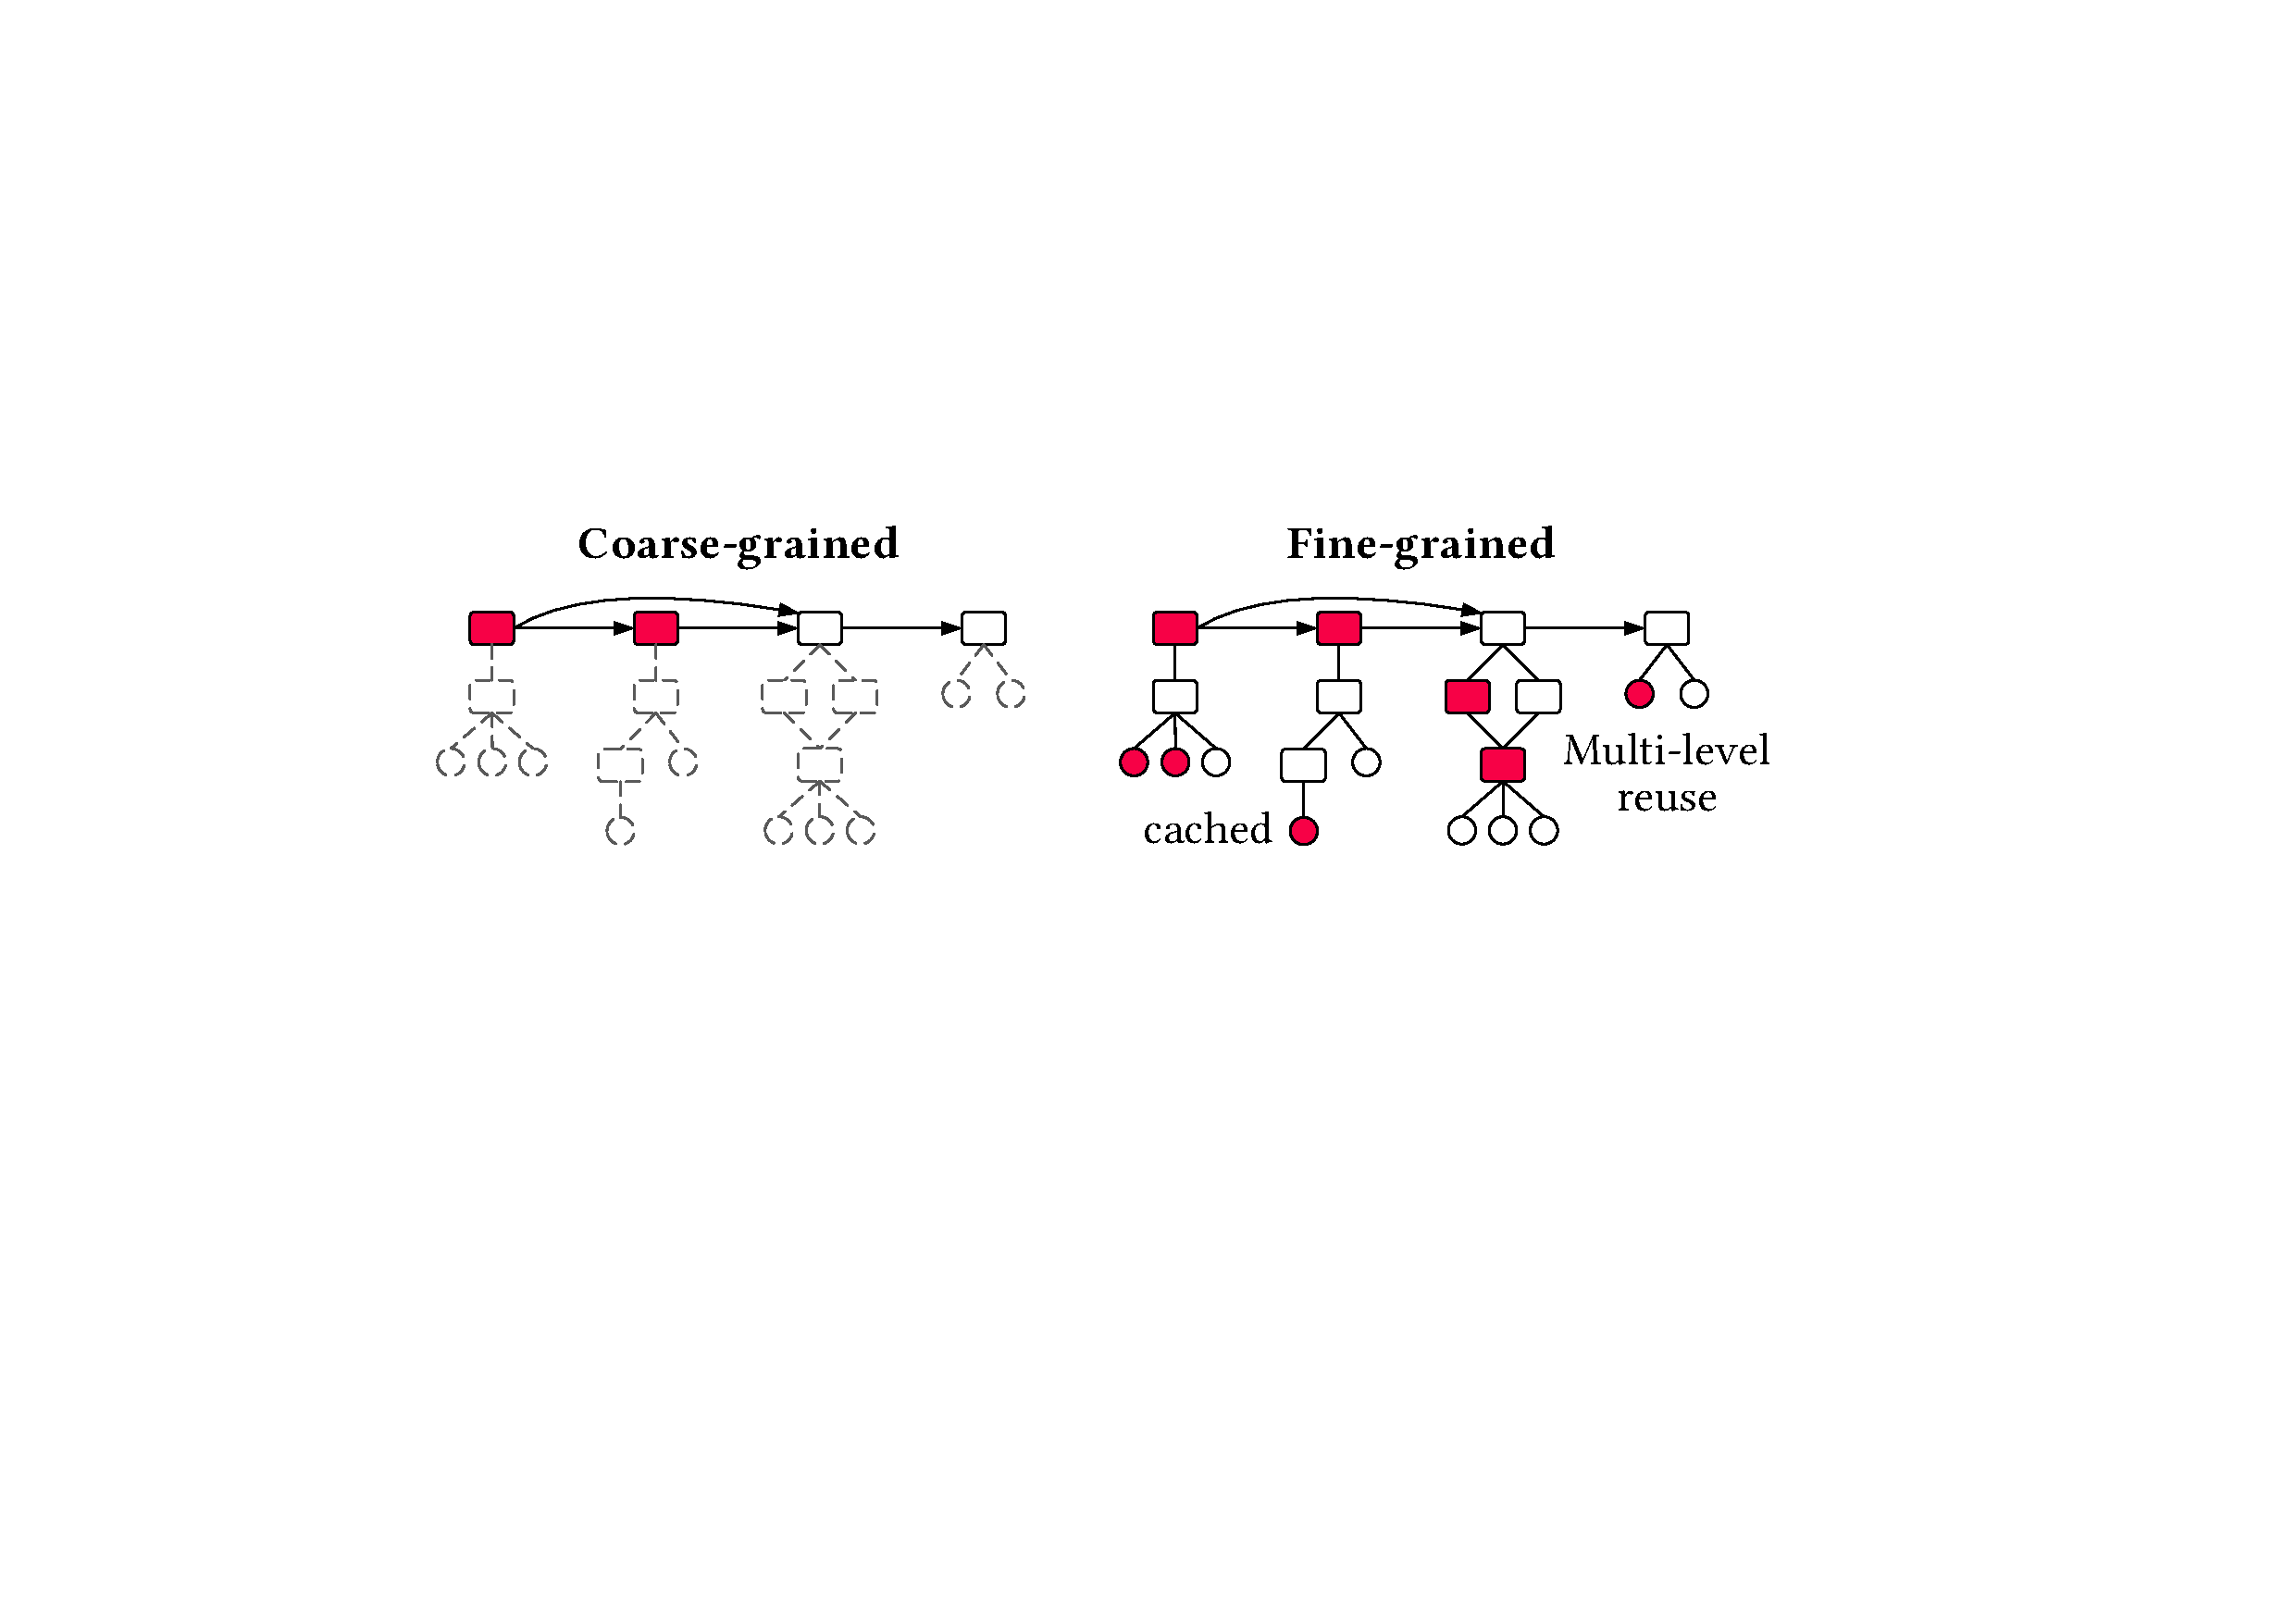
\includegraphics[scale=0.317]{figures/coarse_vs_fine2}
	\vspace{-0.25cm}
	\caption{\label{fig:coarsefine}Coarse- and Fine-grained Lineage-based Reuse {\normalfont(for ML pipelines, utilizing hierarchically composed building blocks)}.}
	\vspace{-0.1cm}
\end{figure}

% Problem 1: versioning, reproducibility, model management
\textbf{Problem of Non-Determinism:} Many ML primitives are non-deterministic, so multiple runs with the same inputs do not yield the same results. Examples are (1) ML algorithms with randomly initialized models, (2) random reshuffling of matrices for mini-batch algorithms, cross validation, data partitioning, and splitting, (3) drop-out layers for regularization in deep neural networks (DNNs), and (4) basic randomized operations like \texttt{rand} or \texttt{sample}. Interestingly, recent work has found significant impact of random seeds on the model accuracy of cutting-edge DNNs \cite{abs-2002-06305}. When computing lineage for high-level primitives, this internal non-determinism---unless exposed via seed parameters---quickly becomes invisible. Externally encoding this metadata is possible but again defeats the purpose of being independent of underlying ML systems and their implementation. Therefore, non-determinism limits the use of coarse-grained lineage for versioning, reproducibility, and reuse.

% Problem 2: lots of unnecessary redundancy
\textbf{Problem of Unnecessary Redundancy:} The repetitive nature of exploratory data science processes, and increasingly complex, hierarchically composed ML pipelines and workflows, create high computational redundancy. While coarse-grained reuse can eliminate redundancy of identical steps, it fails to eliminate fine-grained redundancy. First, existing ML libraries and systems often compose high-level primitives from smaller building blocks to ensure reuse and consistency. For example, Scikit-learn \cite{PedregosaVGMTGBPWDVPCBPD11} allows creating custom pipelines (via \texttt{make\_pipeline()}) from sequences of pre-processing steps and ML algorithms, and then feed these pipelines into high-level primitives like \texttt{GridSearchCV}. Since this composition is unaware of independent operations and substeps, (and hand-optimized primitives for all combinations are infeasible), we end up with unnecessary redundancy. Unfortunately, in general-purpose programming languages, this redundancy is very difficult to correctly detect and eliminate. Second, entire ML algorithms might be repeatedly used inside feature selection and cross validation primitives, which show an orthogonal type of partial redundancy due to incrementally added features (feature selection), removed features (debugging), or overlapping fold compositions.  

\textbf{LIMA Framework Overview:} Our LIMA framework overcomes these problems by a novel concept of \emph{fine-grained} lineage tracing and reuse \emph{inside} ML systems, as shown in Figure~\ref{fig:coarsefine}-right. We maintain a lineage DAG (directed acyclic graph) for all life variables during runtime of an ML program. Nodes represent executed operations---including parameters that make them deterministic (e.g., system-generated random seeds)---and edges are data dependencies. This DAG is recursively built, while executing conditional control flow and operations. The lineage of a variable exactly identifies an intermediate result, and can then be accessed, stored, and used to reproduce this intermediate. In order to eliminate unnecessary redundancy, we further leverage the lineage as keys in a reuse cache for full and partial reuse, with compensations for partial reuse. Figure~\ref{fig:coarsefine} shows the resulting reuse opportunities at the granularity of individual operations, control-flow blocks, and functions.

\textbf{Contributions:} Our main contribution is the LIMA framework for efficient, fine-grained lineage tracing and reuse, implemented in Apache SystemDS\footnote{The source code is available at \url{https://github.com/apache/systemds}.} \cite{BoehmADGIKLPR20} as a representative ML system. Key ideas of this approach, beyond state-of-the-art, are (1) multi-level lineage tracing and reuse, (2) full and partial reuse of intermediates, and (3) a robust integration with ML system internals such as task parallelism and operator fusion. Our technical contributions are:
\begin{itemize}
\item \emph{ML Systems Background:} To aid understanding, we provide the necessary background of ML system internals, and discuss different sources of redundancy in Section~\ref{sec:bg}.
\item \emph{Lineage Tracing:} We then define the concept of Lineage DAGs, and discuss multi-level lineage tracing in Section~\ref{sec:lic}. This discussion also includes the deduplication of lineage traces for functions, loops, blocks, and fused operators. 
\item \emph{Lineage-based Reuse:} Leveraging these lineage traces, we introduce techniques for full and partial reuse of intermediates in Section~\ref{sec:reuse}. This reuse infrastructure relies on compiler-assisted, cost-based runtime caching, tailor-made eviction policies, and thread-safe access in task-parallel programs.
\item \emph{Experiments:} Finally, we report on extensive experiments in Section~\ref{sec:exp} that show low overhead lineage tracing, and significant performance improvements, compared to baselines like TensorFlow~\cite{AbadiBCCDDDGIIK16} and HELIX~\cite{XinMMLSP18}, on various ML workloads.
\end{itemize}
 
 %Section 1
\section{Background and Preliminaries}
\label{sec:bg}

This section introduces our running example, necessary background of ML system internals, as well as common types of redundancy.

\subsection{Running Example}

Example~\ref{ex:1} shows a user-level example ML pipeline---written in SystemDS' DML scripting language with R-like syntax \cite{BoehmADGIKLPR20}---which we use as a running example throughout this paper.

\begin{example} [GridSearch LM] \label{ex:1} We read a feature matrix \mat{X} and labels \mat{y}, and extract 10 random subsets of 15 features. For each feature set, we tune the linear regression (lm) hyper-parameters regularization, intercept, and tolerance via grid search and print the loss.
\begin{lstlisting}
 1: X = read('data/X.csv'); # 1M x 100
 2: y = read('data/y.csv'); # 1M x 1
 3: for( i in 1:10) {
 4:   s = sample(15, ncol(X));
 5:   [loss, B] = gridSearch('lm', 'l2norm',
        list(X[,s],y), list('reg','icpt','tol'),...);
 6:   print("Feature set ["+toString(s)+"]: "+loss);
 7: }
\end{lstlisting}
High-level primitives like \texttt{gridSearch} and \texttt{lm} are themselves script-based built-in functions and imported accordingly. Below functions show their key characteristics in simplified form:
\begin{lstlisting}
01: gridSearch = function(...) return(...) {
02:   HP = ... # materialize hyper-parameter tuples
03:   parfor( i in 1:nrow(HP) ) { # parallel for
04:     largs = ... # setup list hyper-parameters
05:     rB[i,] = t(eval(train, largs));
06:     rL[i,] = eval(score, list(X,y,t(rB[i,])));
07: } }
08: lm = function(...) return(...) { 
09:   if (ncol(X) <= 1024)  # select closed-form
10:     B = lmDS(X, y, icpt, reg, verbose);
11:   else                  # select iterative
12:     B = lmCG(X, y, icpt, reg, tol, maxi, verbose);
13: } 
14: lmDS = function(...) return(...) {
15:   if (icpt > 0) {
16:     X = cbind(X, matrix(1,nrow(X),1));
17:     if (icpt == 2)
18:       X = scaleAndShift(X); # mu=0,sd=1
19:   } ...
20:   A = t(X) %*% X + diag(matrix(reg,ncol(X),1);
21:   b = t(X) %*% y;
22:   beta = solve(A, b);
23: } 
24: lmCG = function(...) return(...) {
25:   if (icpt > 0) {
26:     X = cbind(X, matrix(1,nrow(X),1));
27:     if (icpt == 2)
28:       X = scaleAndShift(X); # mu=0,sd=1
29:   } ...
30:   while (i<maxi & norm_r2>norm_r2_tgt) {
31:     q = t(X) %*% (X %*% ssX_p); ...
32:     p = -r + (norm_r2 / old_norm_r2) * p;
33: } }
\end{lstlisting}
The \texttt{gridSearch} function enumerates and materializes all hyper-parameter combinations $\mat{HP}$ of the passed parameters and value ranges, and invokes training (\texttt{lm}) and scoring (\texttt{l2norm}) functions to find the best model and loss. The \texttt{lm} function in turn dispatches---based on the number of features---either to a closed-form method with $\mathcal{O}(m\cdot n^2 + n^3)$ complexity (\texttt{lmDS}); or an iterative conjugate-gradient method with $\mathcal{O}(m \cdot n)$ per iteration (\texttt{lmCG}), which performs better for many features as it requires $\leq n$ iterations until convergence.
\vspace{-0.1cm}
\end{example}

\subsection{ML Systems Background}
\label{sec:mlsys}

There is a variety of existing ML systems. Relevant for understanding this paper, are especially the underlying techniques for program and DAG compilation, and operator scheduling~\cite{2019Boehm}. Here, we focus primarily on lazy evaluation and program compilation.

\textbf{Program/DAG Compilation:} We distinguish three types of compilation in contemporary ML systems: (1) interpretation or eager execution, (2) lazy expression or DAG compilation, and (3) program compilation. First, interpretation as used in R, PyTorch \cite{PaszkeGMLBCKLGA19}, or Python libraries like NumPy \cite{WaltCV11} or Scikit-learn \cite{PedregosaVGMTGBPWDVPCBPD11} execute operations as-is and the host language (e.g., Python) handles the scoping of variables. Second, systems like TensorFlow \cite{AbadiBCCDDDGIIK16}, OptiML \cite{SujeethLBRCWAOO11}, and Mahout Samsara \cite{MahoutSamsara} performing lazy expression evaluation that lazily collects a DAG of operations, which is optimized and executed on demand. Some of these systems---like TensorFlow or OptiML---additionally provide control flow primitives, integrated in the data flow graph. Here, the host language still interprets the control flow, and thus, unrolls operations into a larger DAG. However, recent work like AutoGraph \cite{abs-1810-08061} automatically compiles TensorFlow control flow primitives. Only bound output variables leave the scope of expression evaluation. Third, program compilation in systems like Julia \cite{BezansonEKS17}, SystemML \cite{BoehmDEEMPRRSST16}, SystemDS~\cite{BoehmADGIKLPR20}, and Cumulon \cite{HuangB013} compiles a script into a hierarchy of program blocks, where every last-level block contains DAGs of operations. Accordingly, control flow and variable scoping is handled by the ML system itself. Despite the large optimization scope of lazy expression evaluation and program compilation, unnecessary redundancy cannot be fully eliminated via code motion and common subexpression elimination (CSE) because the conditional control flow is often unknown.

\begin{figure}[!t]
	\centering
	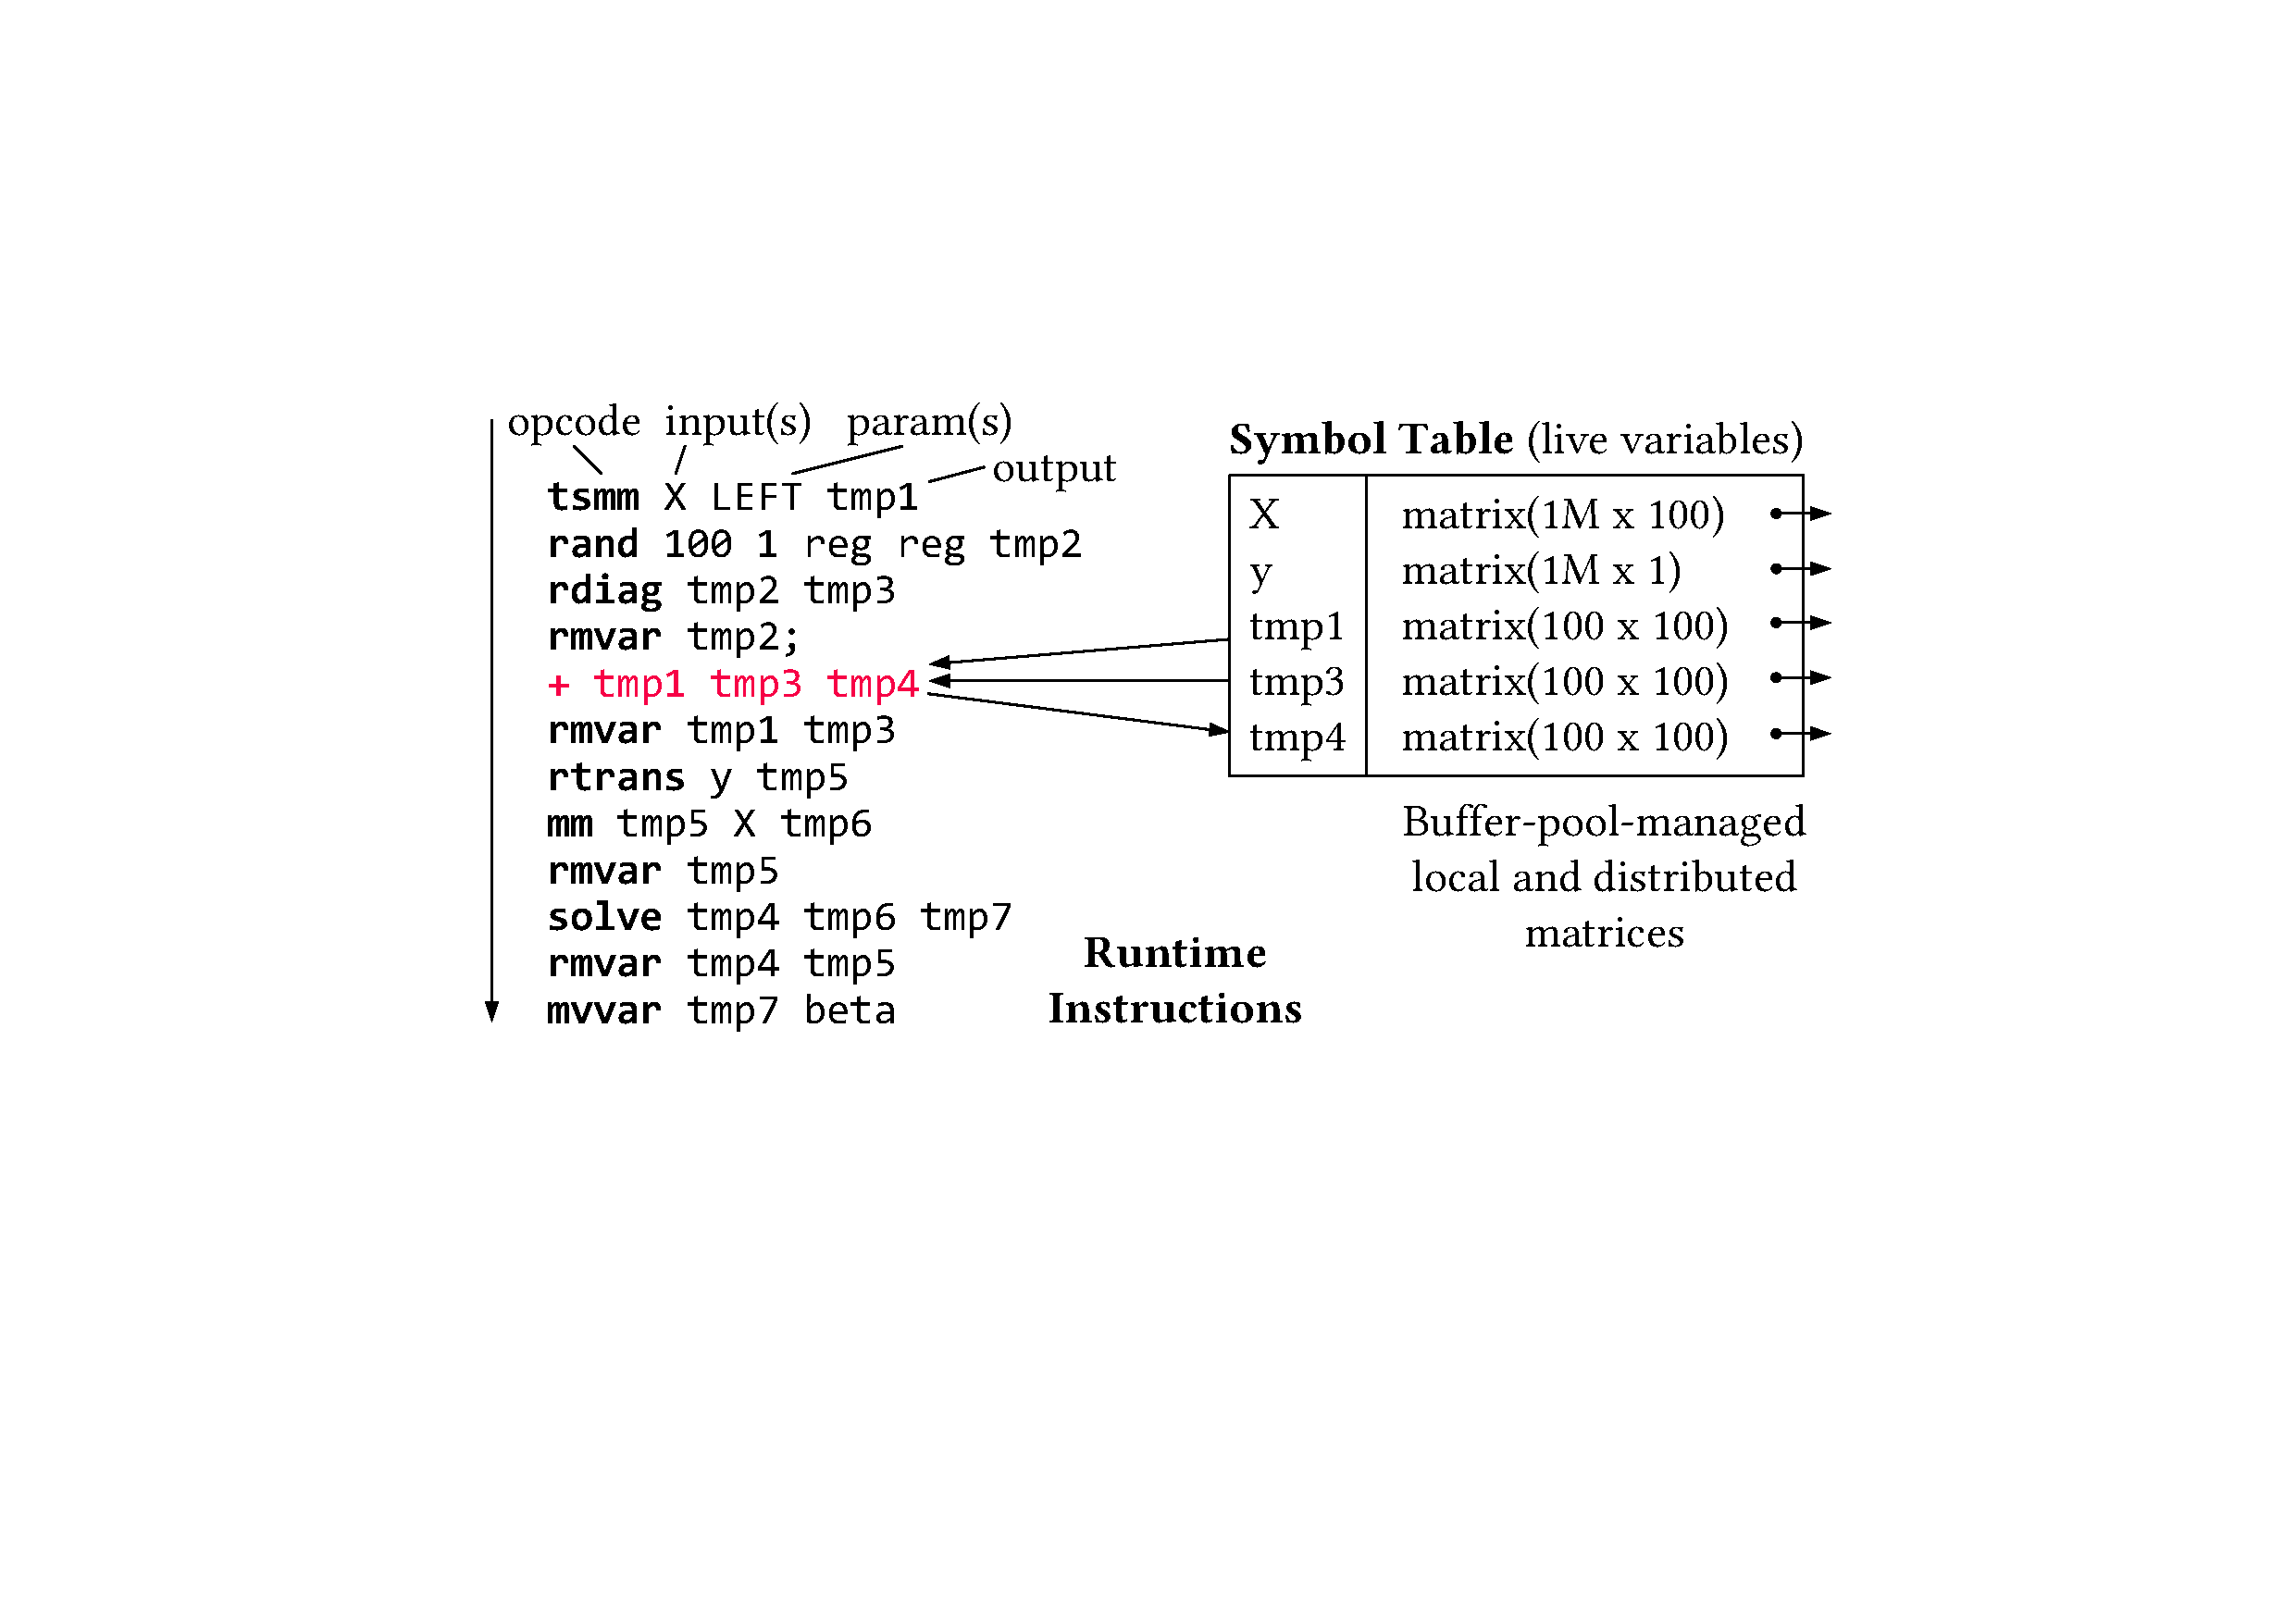
\includegraphics[scale=0.32]{figures/background}
	\vspace{-0.25cm}
	\caption{\label{fig:background}Operator Scheduling and Runtime Plans.}
\end{figure}

\textbf{Operator Scheduling:} Given a DAG of operations of an expression or program block, operator scheduling then determines an execution order of the individual operations, subject to the explicit data dependencies (i.e., edges) of the data flow graph. The two predominant approaches are sequential and parallel instruction streams. First, a sequential instruction stream linearizes the DAG---in depth- or breadth-first order---into a sequence of instructions that is executed one-at-a-time. For example, Figure~\ref{fig:background} shows a plan of runtime instructions in SystemDS for lines 21-23 of Example 1. A symbol table holds references to live variables and their metadata. Instructions are executed sequentially, read their inputs from a variable map (a.k.a. symbol table), and put their outputs back. Such a serial execution model---as used in PyTorch \cite{PaszkeGMLBCKLGA19} and SystemML \cite{BoehmDEEMPRRSST16,BoehmBERRSTT14}---is simple and allows bounding the memory requirements. Second, parallel instruction streams---as used in TensorFlow \cite{AbadiBCCDDDGIIK16}---leverage inter-operator parallelism: when all inputs of an operation are available, this operation is enqueued for parallel execution. This  execution model offers a high degree of parallelism (for many small operations) but makes memory requirements less predictable. 

\subsection{Sources of Redundancy} 
\label{sec:redundancy}

We can now return to our running example and discuss common sources of fine-grained redundancy.

\begin{example} [GridSearch LM Redundancy] 
The user script from Example~\ref{ex:1} with a $1\text{M} \times 100$ feature matrix $\mat{X}$ and three hyper-parameters (\texttt{reg}, \texttt{icpt}, \texttt{tol} with 6, 3, and 5 values) exhibits multiple sources of redundancy. 
%
First, since $\mat{X}$ has 100 features, all calls to \texttt{lm} are dispatched to \texttt{lmDS} and thus, one of the hyper-parameters (\texttt{tol}) is irrelevant and we train five times more models than necessary. 
%
Second, evaluating different $\lambda$ parameters (\texttt{reg}) for \texttt{lmDS} exhibits fine-grained operational redundancy. The core operations $\mat{X}^{\top}\mat{X}$ and $\mat{X}^{\top}\mat{y}$ are independent of \texttt{reg} and thus, should be executed only once for different $\lambda$. 
%
Third, both \texttt{lmDS} and \texttt{lmCG} have the same pre-processing block, and for 2/3 of \texttt{icpt} values, we perform the same \texttt{cbind} operation, which is expensive because it creates an intermediate larger than $\mat{X}$.
%
Fourth, appending a column of ones does not require re-executing $\mat{X}^{\top}\mat{X}$ and $\mat{X}^{\top}\mat{y}$. Instead we can reuse these intermediates and augment them with $\text{colSums}(\mat{X})$, $\text{sum}(\mat{y})$ and $\text{nrow}(\mat{X})$. Similarly, the random feature sets will exhibit overlapping features whose results can be reused.
%
%Overall, eliminating all redundancy allows us to reduce the number of floating point operations from XXX to XXX.
\end{example} 

\textbf{Types of Redundancy:} Existing work performs reuse for coarse-grained sub-tasks in ML pipelines \cite{SparksVKFR17, ZhangKR14, VartakTMZ18, XinMMLSP18, ShangZBKECBUK19, DerakhshanMARM20}. Generalizing upon the previous example, we further extend this to common types of \emph{fine-grained} redundancy:
\begin{itemize}
\item \emph{Full Function or Block Redundancy:} At all levels of the program hierarchy, there is potential for full reuse of the outputs of program blocks. This reuse is a form of function memoization \cite{CrankshawWZFGS17}, which requires deterministic operations. %on the taken control path
\item \emph{Full Operation Redundancy:} Last-level operations can be reused for equivalent inputs, given that all non-determinism (e.g., a system-generated seed) is exposed from these operations and cast to a basic input as well.
\item \emph{Partial Operation Redundancy:} Operation inputs with overlapping rows or columns further allow reuse by extraction from---or augmentation of---previously computed results.
\end{itemize}
Together, these different types of redundancy motivate a design with (1) fine-grained lineage tracing, (2) multi-level, lineage-based reuse, and (3) exploitation of both full and partial reuse.

\textbf{Applicability in ML Systems:} Fine-grained lineage tracing and reuse is applicable in ML systems with eager execution, lazy  evaluation, and program compilation. In contrast, multi-level tracing, deduplication, and reuse require access to control structures and thus, are limited to systems with program compilation scope.
   %Section 2
\section{Lineage Tracing}
\label{sec:lic}

As a foundation of lineage-based reuse, we first describe efficient means to lineage tracing and key operations. Lineage graphs may get very large though, especially for mini-batch training. For this reason, we introduce the idea of lineage deduplication for loops and functions. Finally, we discuss design decisions and limitations.

\subsection{Basic Lineage Tracing}
\label{sec:tracing}

During runtime of a linear algebra program, LIMA maintains---in a thread- and function-local manner---lineage DAGs for all live variables of this execution context. Figure~\ref{fig:lineage} shows the lifecycle of such lineage information and key operations.

\begin{definition2}[Lineage DAGs] A lineage DAG $\mathcal{L}$ is a directed, acyclic graph, whose nodes (or lineage items) represent operations and their outputs, and whose edges represent data dependencies. Lineage items consist of an ID, an opcode, an ordered list of input lineage items, an optional data string and hash, and a visited flag for memoization of processed sub graphs. Leaf nodes are literals or matrix creation operations (e.g., \texttt{read} or \texttt{rand}), and multiple inner nodes might refer to the same inputs. Thus, the lineage DAG is a data flow graph, that encodes the exact creation process of intermediate results, without the computation that determined the control flow path.
\end{definition2}

\textbf{Lineage Tracing:} The immutable lineage DAG for live variables is then incrementally built by lineage tracing as we execute runtime instructions (Figure~\ref{fig:lineage}, \emph{trace}). Every execution context maintains a \texttt{LineageMap} that maps live variable names to lineage items (Figure~\ref{fig:lineage}, red root nodes), and caches literal lineage items. As a lean runtime integration, individual instructions---in a class hierarchy of instructions for local and distributed operations---implement a dedicated interface \texttt{LineageTraceable} for obtaining lineage items. Before\footnote{Lineage tracing \emph{before} instruction execution facilities reuse as described in Section~\ref{sec:reuse}.} executing an instruction (integrated in \texttt{preprocessInstruction}), we obtain the lineage items for the instruction output(s) and update the lineage map. Special instructions like \texttt{mvvar} and \texttt{rmvar}---for renaming and removing variables---only modify the mapping of live variables to lineage items. For capturing non-determinism, we also modified selected runtime instructions, like \texttt{rand} or \texttt{sample}, to create system-generated seeds on \texttt{preprocessInstruction} for inclusion in the lineage items.

\textbf{Comparisons:} When working with multiple, potentially overlapping lineage DAGs, a key operation is the comparison of two lineage DAGs for equivalence or containment (Figure~\ref{fig:lineage}, \emph{compare}). For this purpose, lineage items implement \texttt{hashCode()} and \texttt{equals()}, whose semantics are recursively defined. First, the hash code of a lineage item is computed as a hash over the hashes of the opcode, data item, and all inputs. As lineage DAGs are immutable, we cache the computed hash for every lineage item. Second, the equals check returns true if the opcode, data item, and all inputs are equivalent. In order to handle large DAGs, we use memoization to avoid redundant processing of sub-DAGs reachable over multiple paths, and non-recursive, queue-based function implementations.  

\textbf{Serialization and Deserialization:} Users may obtain the lineage in two forms. First, a new \texttt{lineage(X)} built-in function returns the lineage DAG of variable $\mat{X}$ as a string. Second, for every write to a file \texttt{write(X,'f.bin')}, we also write the lineage DAG to a text file \texttt{'f.bin.lineage'}. Both cases require the serialization of the lineage DAGs (Figure~\ref{fig:lineage}, \emph{serialize}). This serialization unrolls the lineage DAG in a depth-first manner, creating a text line per lineage item. Inputs are represented via IDs and memoization ensures that every item is serialized once in the lineage log. To handle large DAGs, we again use a non-recursive implementation with stack-based data structures. The lineage log can be deserialized back into a lineage DAG (Figure~\ref{fig:lineage}, \emph{deserialize}) by processing the lineage log line-by-line. For every line, we obtain input items from a lookup table, create the lineage item, and store it in the lookup table.

\textbf{Re-computation from Lineage:} Additionally, we provide a utility for generating a runtime program from a lineage DAG (Figure~\ref{fig:lineage}, \emph{reconstruct}) that computes---given the same input---exactly the same intermediate. In contrast to the original program, the reconstructed program does not contain control flow but only the operations for computing the output. The entire lifecycle from tracing, over serialization and deserialization, to the re-computation by lineage is very valuable as it simplifies testing, debugging, and reproducibility as illustrated by the following example.

\begin{example}[Debugging with Lineage] Let us share a debugging story from practice, which motivated the lineage support in SystemDS. Users deployed a sentence classification pipeline in production, noticed differences in results compared to the development setup, and reported this as a blocking issue. We reproduced the setup, spent nights debugging it up to round-off errors of different degrees of parallelism, and yet, still could not reproduce it. Finally, we found that the modified deployment infrastructure passed arguments incorrectly, making the pipeline use default parameters. With lineage support, such multi-person debugging efforts become much simpler: lineage logs can be exchanged, compared, and used to reproduce results.
\end{example}

\begin{figure}[!t]
	\centering
	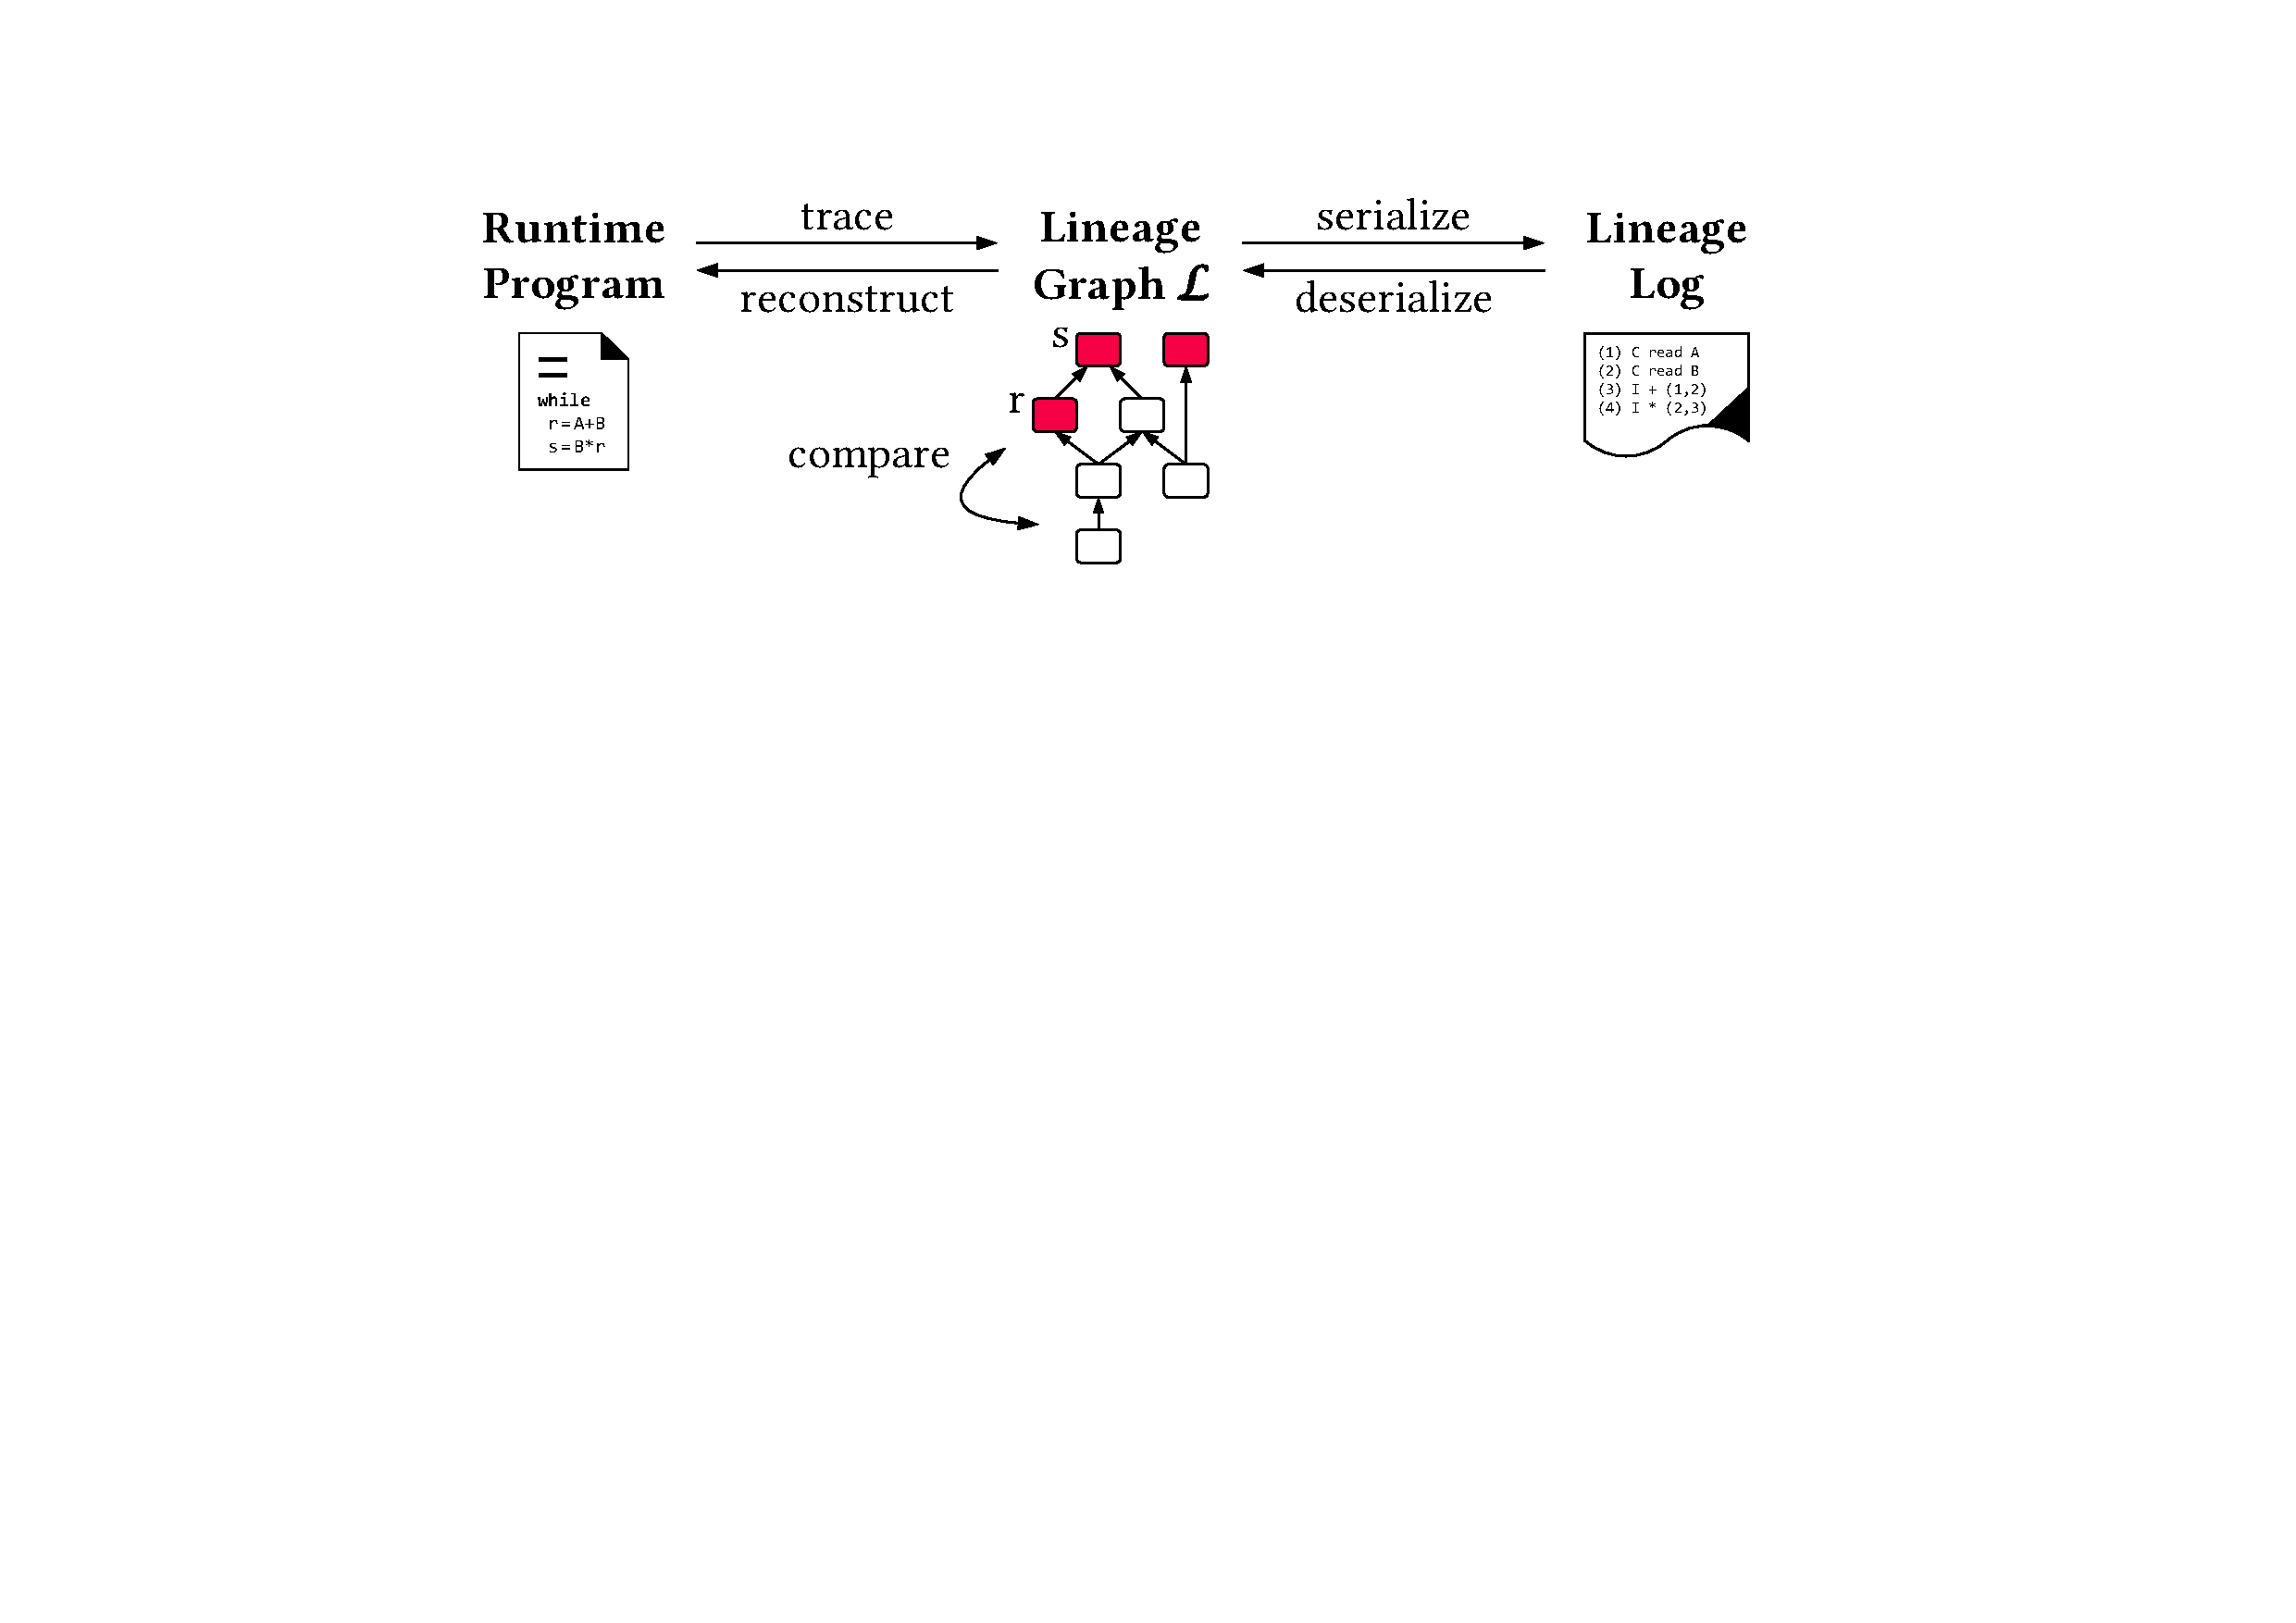
\includegraphics[scale=0.32]{figures/lineage}
	\vspace{-0.25cm}
	\caption{\label{fig:lineage}Lineage Tracing Lifecycle and Operations.}
\end{figure}

\subsection{Lineage Deduplication}
\label{sec:deduplication}

A new challenge of fine-grained lineage tracing are potentially very large lineage DAGs in use cases like mini-batch training. Consider an average lineage item size of $64\bb$, and training 200 epochs on a dataset of $10\text{M}$ rows, batch-size 32, and $\num{1000}$ instructions per iteration. The resulting lineage DAG would grow to $4\tb$. We address this issue inside ML systems with a new concept of \emph{lineage deduplication}, reducing the size to $4\gb$ in this example. Additionally, deduplication can remove the overhead of repetitive tracing.

\textbf{Basic Idea:} Large lineage DAGs originate from the repeated execution of code paths in loops and functions, which create repeated patterns in the lineage graph. The basic idea of lineage deduplication is to eliminate these repeated patterns in the lineage DAG as a form of compression. Conceptually, we extract lineage sub-DAGs called patches, store them once, and refer to these patches via a single lineage item. Since reactive deduplication (after lineage tracing)---similar to function outlining---is a hard problem and brittle, we perform proactive deduplication on entering last-level loops and functions. However, as the number of lineage patches is exponential in the number of branches, we use a \emph{hybrid} design with proactive setup, and minimal runtime tracing.

\textbf{Loop Deduplication Setup:} On entering a last-level \texttt{for}, \texttt{parfor}, or \texttt{while} loop, we analyze the distinct control paths to aid deduplication. The distinct control paths are all possible execution paths (e.g., $2^3$ paths for a sequence of three \texttt{if-else}-blocks), each with its own lineage patch. During setup, we count these paths in a single pass through the program, replicating the current set of traced paths at every branch. In this process, we also assign branch positions (IDs) and materialize these IDs in the \texttt{if-else} program blocks. For nested branches, the IDs are assigned in a depth-first order of the entire subprogram. Additionally, we obtain the inputs and outputs of the loop body from live variable analysis, and prepare an empty map of lineage patches but do not materialize these patches to avoid unnecessary setup for paths that are never taken.

\textbf{Loop Deduplication Tracing:} During iteration runtime, we trace temporary lineage DAGs. We first construct ordered placeholder items for the loop inputs and indexes. Additionally, we initialize a bitvector \mat{b} for tracing the taken path, where bit $\mat{b}_i$ is set to the evaluated condition of branch $i$. We then execute the loop body, while performing basic lineage tracing and updating \mat{b}. At the end of an iteration, we maintain the map of lineage patches and the global lineage DAG. The bitvector \mat{b} represents the key of the lineage patch, and we keep the collected lineage DAG as a new patch if it does not yet exist. Finally, a single dedup lineage item---pointing to the lineage patch---is added onto the global lineage DAG. Once lineage patches are created for all distinct paths, we stop this on-demand lineage tracing, and only trace the taken control paths.

\begin{figure}[!t]
	\centering
	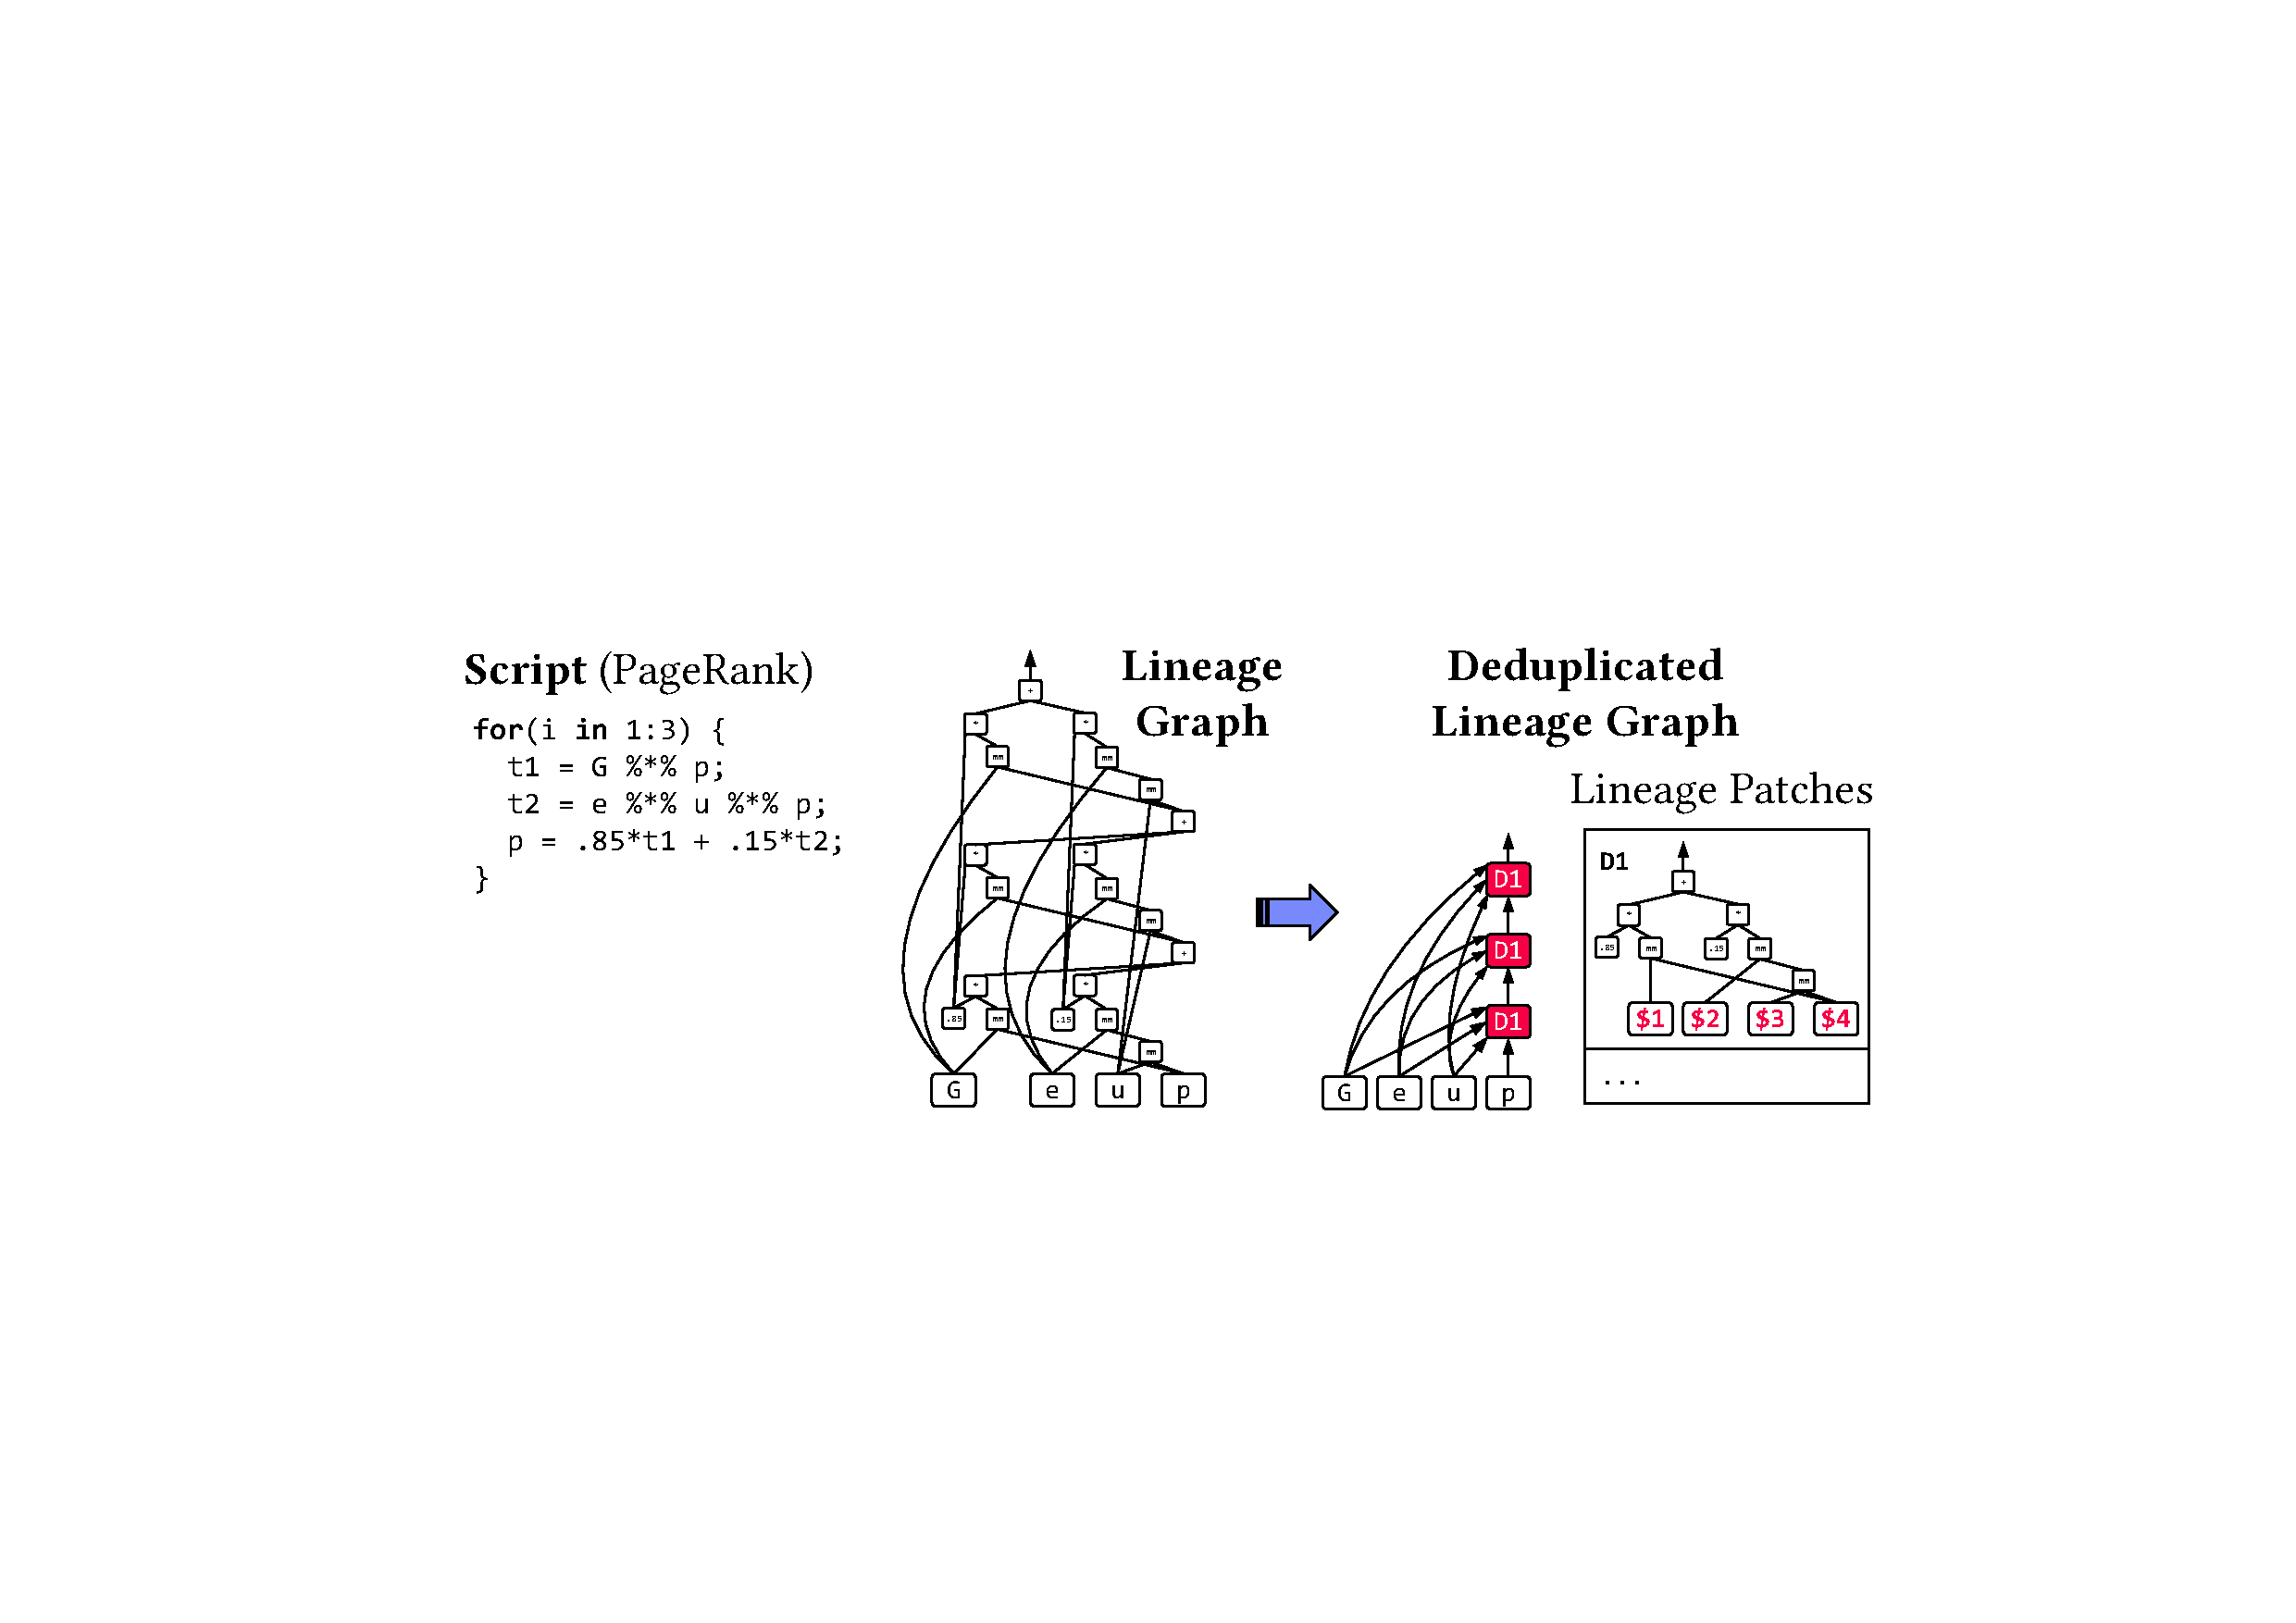
\includegraphics[scale=0.32]{figures/dedup}
	\vspace{-0.25cm}
	\caption{\label{fig:dedup}Example Lineage Deduplication for PageRank.}
\end{figure}

\begin{example}[PageRank Loop Deduplication] Figure~\ref{fig:dedup} illustrates this concept of loop deduplication for a classical PageRank graph algorithm. On the left, we see the original script, where $\mat{G}$ is a sparse graph representing the linked websites, and $\mat{p}$ is the iteratively updated page rank of individual sites. When executing three iterations without deduplication, we get the lineage graph in the center with repeated substructures. In contrast, with loop deduplication, we have extracted one lineage patch with four inputs and one output, and add a single lineage item per iteration to the lineage graph.
\end{example}

\textbf{Function Deduplication:} Similar to loop deduplication, we apply the same concept for functions that do not contain loops or other function calls. We again count the distinct control paths upfront, use the bitvector approach to trace the taken path, and add a single lineage item per function call to the lineage graph. Additional support for nested loops and function calls is interesting future work. We focused on last-level loops and functions, which offers a good tradeoff between simplicity and benefit of deduplication.

\textbf{Handling of Non-Determinism:} Coming back to our example of mini-batch training. Many DNN architectures contain \texttt{dropout} layers for regularization, which is a non-deterministic operation that generates new dropout masks in every iteration. Our approach to handling such non-determinism in the context of deduplication is to model the seeds as input placeholders of the lineage patch, trace these seeds like the control path bitvector, and add them as literal inputs to the single dedup item. Similarly, all functions are tagged as deterministic or non-deterministic during compilation.

\textbf{Operations on Deduplicated Graphs:} All basic lineage operations apply to deduplicated lineage graphs too. However, na\"ively decompressing the lineage graph---by lookup of lineage patches and expansion---would defeat the purpose of deduplication. We alleviate this problem by two extensions. First, we \emph{serialize} and \emph{deserialize} the dictionary of lineage patches to preserve the deduplication for storage and transfer. We further extended the \emph{compare} functionality to match normal and deduplicated sub-DAGs, by enforcing equal hashes for regular and dedup items, and resolving dedup items if needed. Second, program reconstruction would also cause expansion. Hence, on \emph{reconstruct}, we compile the lineage patches into functions, and sequences of equivalent dedup items into loops.

\subsection{Lineage Tracing for Advanced Features}
\label{sec:advanced}

Modern ML systems further provide advanced features such as (1) operator fusion, and (2) task-parallel for loops, which are both widely used and thus, important to integrate with lineage tracing.

\textbf{Operator Fusion:} Operator fusion via code generation is crucial for performance because it can avoid materialized intermediates \cite{CrottyGDKBCZ15,BoehmRHSEP18,PalkarTNTPNSSPA18}, allow scan sharing and sparsity exploitation \cite{BoehmRHSEP18,HuangB013}, and kernel specialization for accelerators \cite{ChenMJZYSCWHCGK18,XLA,AshariTBRCKS15}. However, fusion loses the operator semantics and thus, does not allow lineage tracing. This limitation is problematic because it cuts the lineage trace into unusable pieces. Our approach is simple, yet effective. We construct the lineage patches of fused operators (with ordered placeholders) during compilation, and store them in a dictionary. During runtime, we expand the lineage graph by these lineage patches. Lineage now also enables new techniques such as de-optimizing fused operators and reuse-aware fusion.
  
\textbf{Task-parallel Loops:} Numerical computing frameworks like MATLAB~\cite{SharmaM09}, R~\cite{Rdopar}, or Julia~\cite{BezansonEKS17}, and ML systems like TensorFlow~\cite{AbadiBCCDDDGIIK16} or SystemML~\cite{BoehmDEEMPRRSST16,BoehmTRSTBV14} provide means of task-parallel loops (e.g., for hyper-parameter tuning). Implementation details vary, but often multi-threaded and/or distributed workers are used. For ensuring isolation, we trace lineage in a worker-local manner, but individual lineage graphs share their common input lineage. Distributed operations leverage the \emph{serialize} and \emph{deserialize} operations to transfer lineage. The worker results are merged by taking their lineage roots and constructing a linearized lineage graph.

\subsection{Limitations}
\label{sec:limits1}

The LIMA lineage tracing makes several tradeoffs. In the following, we discuss these design decisions and related limitations.
\begin{itemize}
\item \emph{Immutable Files/RDDs:} We assume input files and RDDs are read-only (i.e., deterministic reads), which is a reasonable assumption and eliminates the need for data summarization. 
\item \emph{No Capturing of Control Flow:} The lineage DAG represents the computation of an intermediate without the control path decisions. We made this choice because the original script is a more concise representation of the actual program.
\item \emph{Result Differences:} Despite handling non-determinism, reconstructed programs might produce slightly different results. Reasons include multi-threaded or distributed operations (aggregation orders), different environments (memory budgets, cluster size), and different artifacts (SW versions).
\end{itemize}
Our design focuses primarily on simplicity, efficiency, and robustness, which are key for leveraging lineage in many use cases like versioning, debugging, auto differentiation, and lineage-based reuse. 

%TODO deduplication with non-determinism (seed placeholders) 
%TODO deduplication for functions
      %Section 3
\section{Lineage-based Reuse}
\label{sec:reuse}

The lineage of an intermediate carries all information to identify and recompute this intermediate. LIMA leverages this characteristic in a lineage-based reuse cache for eliminating fine-grained redundancy (see Section~\ref{sec:redundancy}). Figure~\ref{fig:reuse} gives an overview of our reuse approach. In this section, we describe (1) the lineage cache organization, and multi-level reuse of intermediates for functions, blocks, and operations, (2) partial reuse of operations with compensations, (3) cost-based eviction policies, (4) compiler-assisted reuse (e.g., rewrites), and (5) remaining limitations and future work.

\subsection{Multi-Level Full Reuse}
\label{subsec:mlreuse}

As the foundation of lineage-based reuse, we establish a cache that maps lineage traces to cached, in-memory data objects. Here, we describe a holistic design for a robust system integration.

\textbf{Lineage Cache:} The basic architecture of the lineage cache---as shown in Figure~\ref{fig:reuse}---comprises a hash map from lineage items (i.e., lineage traces of values) to cached values. These values can be matrices, frames, or scalars and are wrapped into lineage cache entries that hold additional metadata such as the data type, cache status, computation time, access timestamps, and eviction scores. The cache size is a configurable fraction of the maximum heap size (5\% by default). Other configurations include the set of reusable instruction opcodes, the used eviction policy, and related parameters.

\textbf{Full Reuse:} During runtime, we then trace lineage \emph{before} instruction execution, and use the obtained lineage item to probe the lineage cache for existing outputs. Full reuse refers to an operation-level reuse of a previously computed output in full, that is, without any compensations. If this probe succeeds, we obtain the cached value, put this value into the symbol table of live variables, and skip the instruction. If the value does not yet exist in the cache, we execute the instruction and additionally store its output(s) in the lineage cache. The probing leverages the \emph{compare} functionality (via \texttt{hashCode()} and \texttt{equals()}) as described in Section~\ref{sec:tracing}. The time complexity of na\"ive \texttt{hashCode} and \texttt{equals} implementations are linear in the size of the lineage trace. However, due to materialized hash codes, we get constant complexity for constructing and hashing a new lineage item over existing lineage inputs, and using the hash codes for pruning\footnote{Long lineage traces with repeated structure are prone to hash collisions due to integer overflows. We handle such overflows with separate hash functions.}---in \texttt{equals} calls---works very well in practice. The reuse logic is integrated in the main instruction execution code path, which seamlessly applies to all instructions. In addition, making the set of cacheable instructions and data types configurable also avoids unnecessary cache pollution, and ensures correctness (e.g., for update-in-place indexing). 

\begin{figure}[!t]
	\centering
	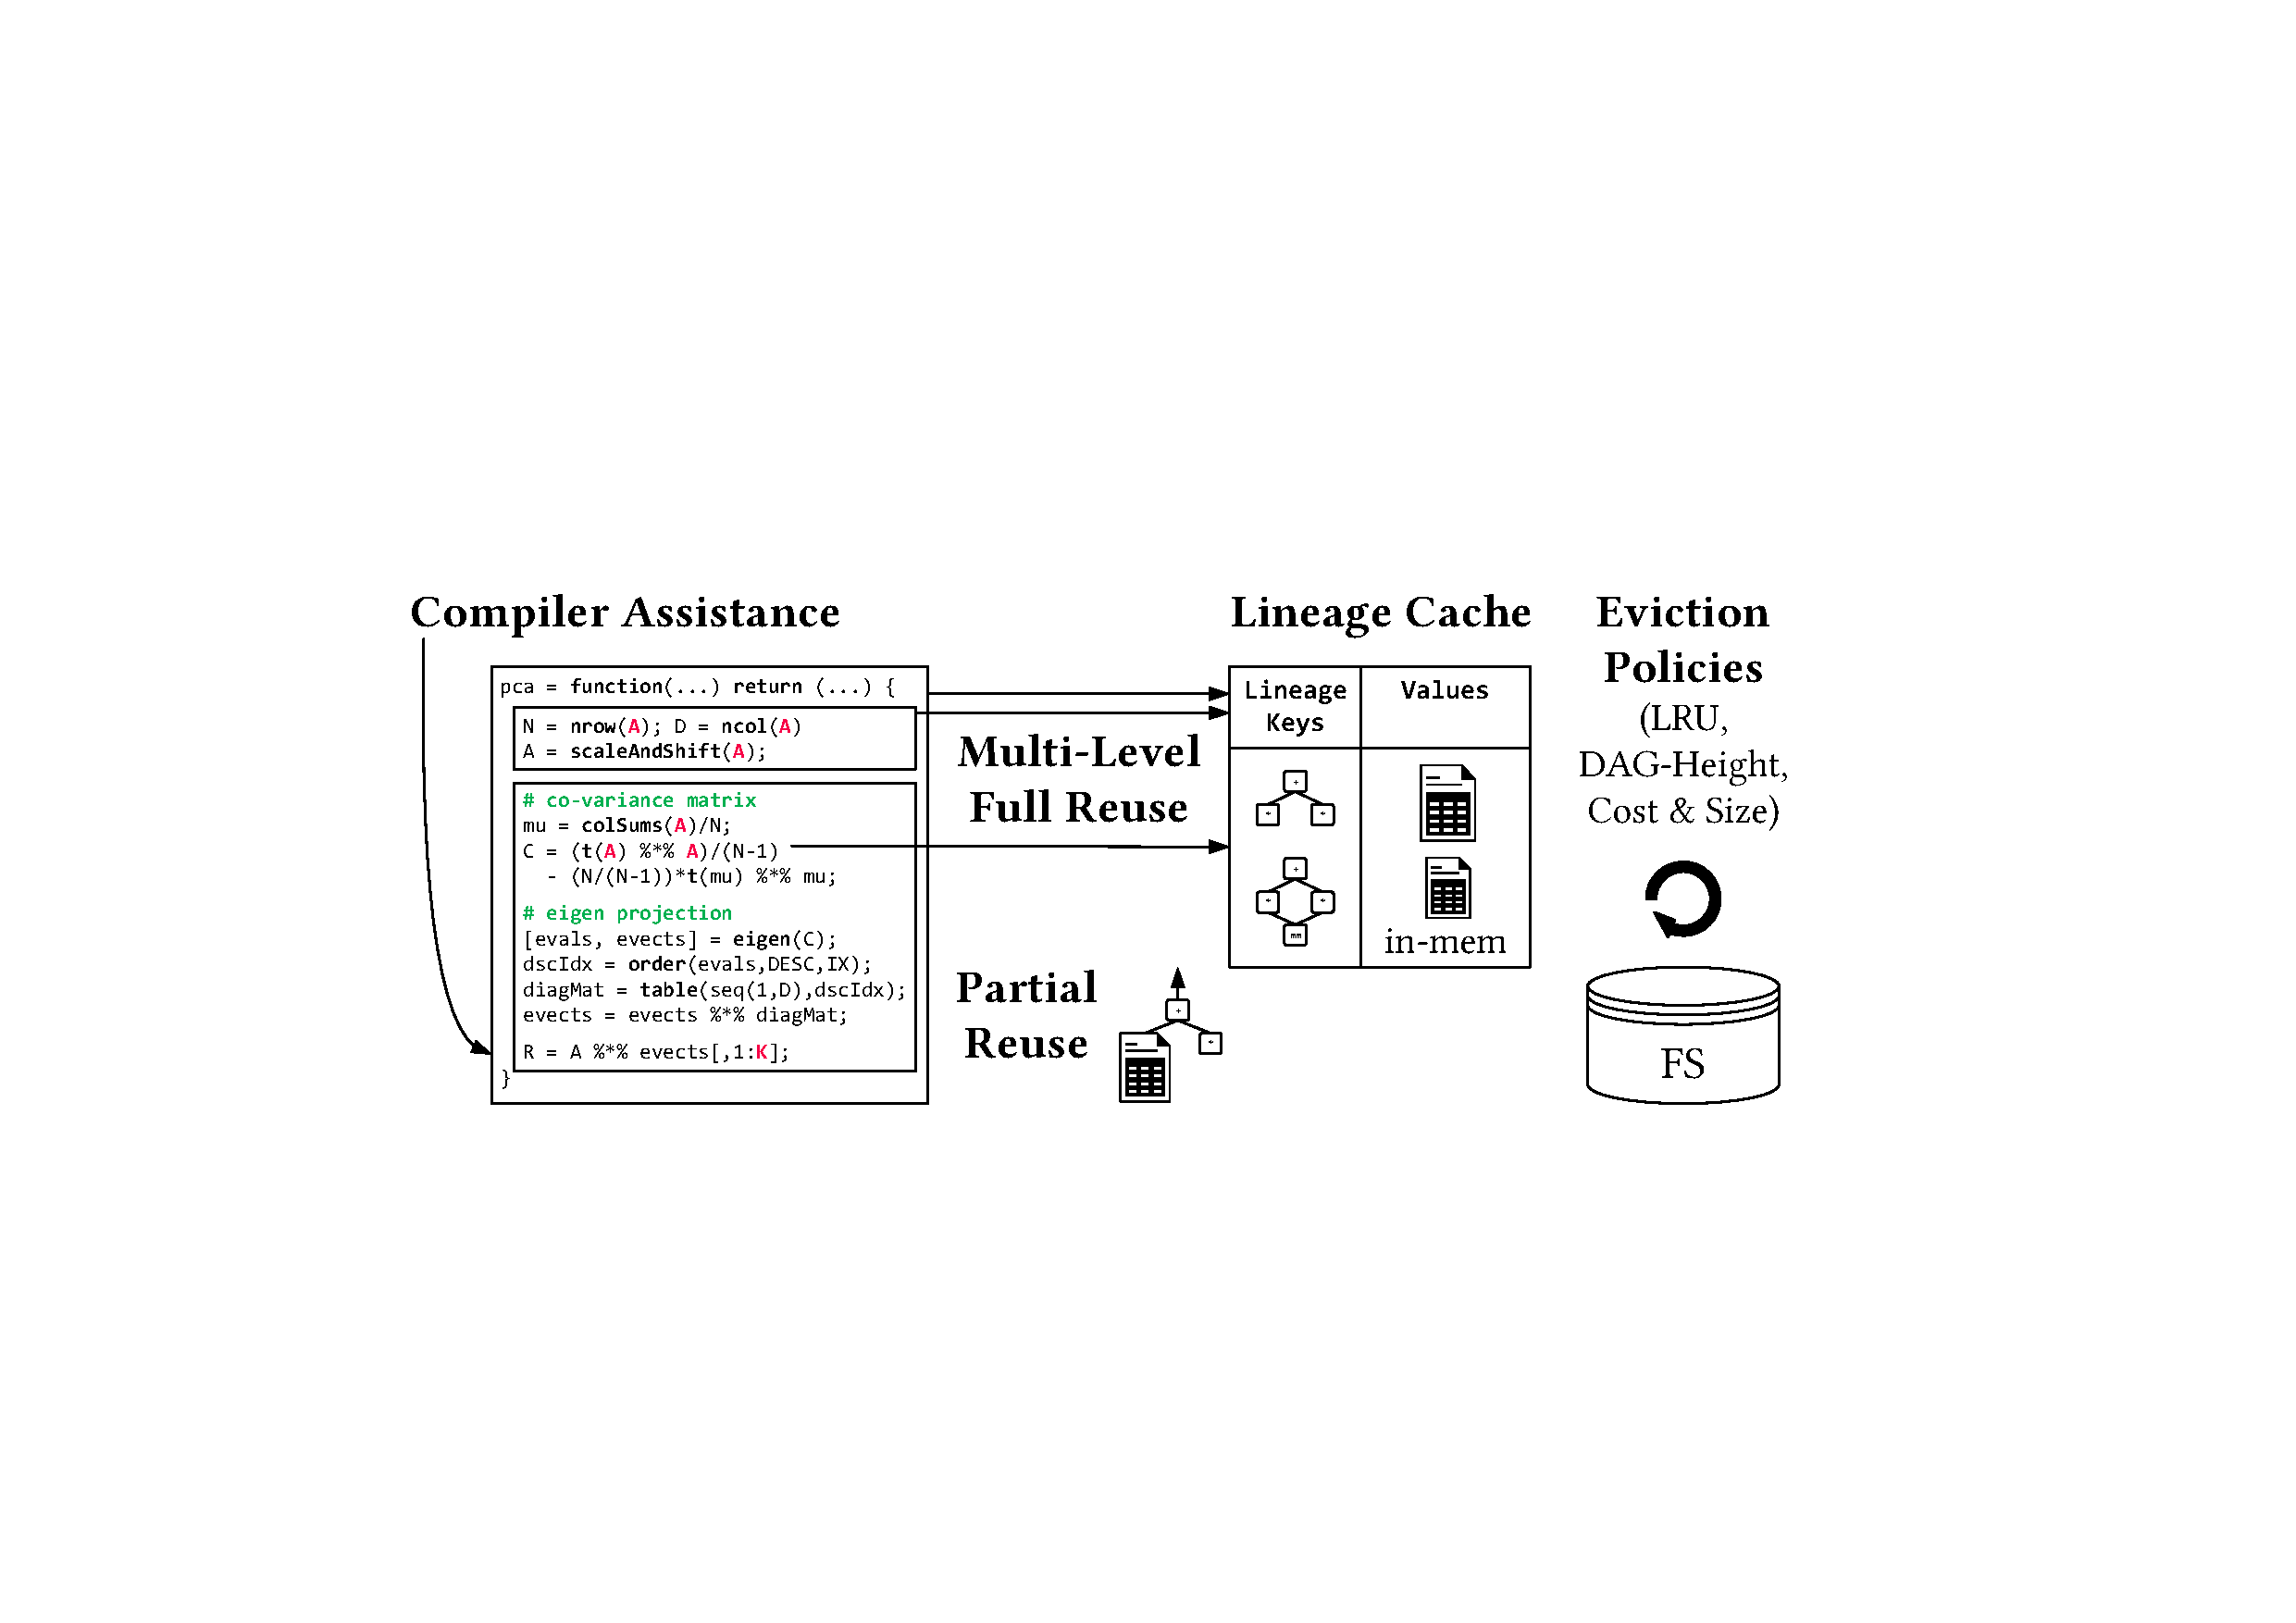
\includegraphics[scale=0.32]{figures/reuse}
	\vspace{-0.25cm}
	\caption{\label{fig:reuse}Overview Lineage-based Reuse.}
\end{figure}

\textbf{Multi-level Reuse:} Our basic full reuse eliminates fine-grained redundancy at operation level in a robust manner. However, this approach is suboptimal for coarse-grained redundancy (e.g., reuse of entire functions) because it still requires a pass over all instructions and reuse of their  cached outputs. Inspired by recent work on alternative probing strategies in CO~\cite{DerakhshanMARM20} and pruning in HELIX~\cite{XinMMLSP18}, we augment the basic reuse by a multi-level reuse approach to avoid cache pollution and interpretation overhead. Our basic idea is to leverage the hierarchical program structure of functions and control flow blocks (see background in Section~\ref{sec:mlsys}) as natural probing and reuse points. As pre-processing step, we determine and materialize if a given function or block is deterministic, i.e., does not include any non-deterministic operations or function calls. A block is similar to a function as it has specific inputs and outputs, which we obtain from live variable analysis. During runtime, we then construct a special lineage item that represents the function inputs, function call, and bundles all function outputs. If a deterministic function is called with the same inputs, we can thus, directly reuse its outputs; otherwise we execute the function and also bind cached outputs to the special lineage item. Multi-level reuse is orthogonal to lineage deduplication, but internally leverages shared infrastructure.

\begin{example}[PCA Multi-level Reuse] Figure~\ref{fig:reuse} also illustrates this concept of multi-level reuse, where we first probe the entire \texttt{pca} (principal component analysis) function call. If we cannot reuse, we probe individual blocks (e.g., the block around \texttt{scaleAndShift}), and finally, individual operations (e.g., $\mat{A}^{\top}\mat{A}$ as used in \texttt{pca} and \texttt{lmDS}).
\end{example}

\textbf{Task-parallel Loops:} Similar to lineage tracing, supporting task-parallelism requires further lineage cache extensions. First, multi-threaded \texttt{parfor} workers concurrently probe and update the shared lineage cache. This concurrency requires a thread-safe lineage cache, which we ensure via latches and a careful implementation that keeps the critical sections small and prevents deadlocks. Second, we use lineage cache ``placeholders'' (empty lineage cache entries) to avoid redundant computation in parallel tasks. For example, consider the following hyper-parameter tuning loop:
\begin{lstlisting}
 1: parfor(i in 1:nrow(lambda))
 2:   B[,i] = lmDS(X=X, y=Y, reg=lambda[i,1]);
\end{lstlisting}
For instance, k=32 iterations might run in parallel here, and during the first wave of iterations $\mat{X}^{\top}\mat{X}$ and $\mat{X}^{\top}\mat{y}$ are not yet available for reuse. This redundancy matters because we should rather spend the parallelism in individual operations if needed. Hence, the first thread puts a placeholder in the cache. Other threads then find this placeholder and block on obtaining its matrix, frame, or scalar until the first thread adds the computed value back to the placeholder.


\subsection{Partial Operation Reuse}
\label{sec:partial}

Beyond multi-level full reuse, LIMA also eliminates \emph{partial operation redundancy} via partial reuse. Partial reuse refers to an operation-level reuse of a previously computed output, augmented by a compensation plan of reused or computed operations. 

%TODO only if large enough

\textbf{Partial Reuse:} If full reuse is not possible, we quickly probe different partial reuse opportunities, and only if none applies, fallback to normal instruction execution. This probing for partial reuse evaluates an ordered list of rewrites of source-target patterns. If the current lineage item (before execution) matches a source pattern, and components of the target pattern are available in the lineage cache, we construct a \emph{compensation plan} to compute the result. Similar to constant folding, we put reusable intermediates of the target pattern into a temporary symbol table, construct an operation DAG for the remaining operations, and then, compile and execute actual runtime instructions to obtain the results. The rewrites are hand-written and can include cost-based constraints. Our existing rewrites focus primarily on real use cases and patterns with \texttt{rbind}, \texttt{cbind}, and indexing in combination with matrix multiplications, column or row aggregates, and element-wise operations.

\textbf{Example Rewrites:} Our set of partial rewrites comprises 14 meta rewrites with internal variants. Below equation shows selected examples, where $\mat{X}\,\mat{Y}$ is a matrix multiply, $\odot$ and $+$ are element-wise multiply and addition, and $\textbf{dsyrk}(\mat{X})$ is a shorthand for $\mat{X}^{\top}\mat{X}$.
\[\begin{split}
\textbf{rbind}(\mat{X},\Delta\mat{X})\,\mat{Y} &\rightarrow \textbf{rbind}(\mat{X}\,\mat{Y}, \Delta\mat{X}\,\mat{Y})\\
\mat{X}\,\textbf{cbind}(\mat{Y},\Delta\mat{Y}) &\rightarrow \textbf{cbind}(\mat{X}\,\mat{Y}, \mat{X}\,\Delta\mat{Y})\\
\mat{X}\,\textbf{cbind}(\mat{Y},\mat{1}) &\rightarrow \textbf{cbind}(\mat{X}\,\mat{Y}, \textbf{rowSums}(\mat{X}))\\
\mat{X}\,(\mat{Y}[,1{\,:\,}k]) &\rightarrow (\mat{X}\,\mat{Y})[,1{\,:\,}k]\\
\textbf{dsyrk}(\textbf{rbind}(\mat{X},\Delta\mat{X})) & \rightarrow \textbf{dsyrk}(\mat{X}) + \textbf{dsyrk}(\Delta\mat{X})\\
\textbf{dsyrk}(\textbf{cbind}(\mat{X},\Delta\mat{X})) & \rightarrow \textbf{rbind}(
	\textbf{cbind}(\textbf{dsyrk}(\mat{X}), \mat{X}^{\top}\Delta\mat{X}),\\
	 &\qquad\quad\textbf{cbind}(\Delta\mat{X}^{\top}\,\mat{X}, \textbf{dsyrk}(\Delta \mat{X})))\\
\textbf{cbind}(\mat{X},\Delta\mat{X}) \odot \textbf{cbind}(\mat{Y},\Delta\mat{Y}) &\rightarrow \textbf{cbind}(\mat{X}\odot\mat{Y},\Delta\mat{X}\odot\Delta\mat{Y})\\
\textbf{colAgg}(\textbf{cbind}(\mat{X}, \Delta\mat{X})) &\rightarrow \textbf{cbind}(\textbf{colAgg}(\mat{X}), \textbf{colAgg}(\Delta\mat{X}))\\
\end{split}\]
Similar rewrites have been used for incremental linear algebra programs \cite{NikolicEK14}, linear algebra simplification rewrites \cite{BoehmBERRSTT14,ElgamalLBETRS17,WangHSHL20,FangSW020,JiaPTWZA19}, and hand-optimized cross validation primitives \cite{KunftKSBRM19}. In contrast, we apply them during lineage-based reuse or recompilation. Application examples are \texttt{lm} and \texttt{scaleAndShift} with and without intercept, cross validation, as well as \texttt{stepLm} \cite{VenablesR02,BoehmADGIKLPR20}, a feature selection algorithm that repeatedly appends additional features.

\subsection{Cache Eviction}
\label{sec:eviction}

Lineage cache eviction ensures that the size of cached objects does not exceed the configured budget. Important aspects are the cache management, and dedicated cost-based eviction policies.

\textbf{Cache Management:} Given an absolute memory budget $B$ (by default, 5\% of heap size), intermediates of size smaller than $B$ are subject to caching. On adding such an object $o$ to the cache, we get its in-memory size $s(o)$ and trigger eviction if the cache size $S + s(o)$ exceeds $B$. Objects under eviction management (excluding empty placeholders), are then added to a priority queue $\mat{Q}$ that orders objects for eviction according to eviction-policy-specific scoring functions. An active eviction then pulls and evicts items in order until the budget constraint $S \leq B$ is met. The eviction of an object is either by deletion or by spilling to disk, where we only spill objects whose re-computation time exceed the estimated I/O time. We perform additional bookkeeping to allow identifying such spilled cache entries. With multi-level reuse, multiple cache entries might refer to the same object but exhibit different costs (e.g., function versus operation). In such scenarios, we defer the spilling of an entry group until all group entries are pulled for eviction.

\textbf{Statistics and Costs:} As a basis for our eviction policies and user-facing statistics, we collect various statistics. On entering the cache, we obtain (1) the measured function or operation execution time $c(o)$ of cached objects, and (2) the height $h(o)$ of related lineage traces (distance from leaves). During cache usage, we further gather (3) the last access timestamp $T_a(o)$, and (4) the number of references (\#hits $r_h$, \#misses $r_m$). Additionally, we estimate (5) the spill (write) and restore (read) times of cached objects. We obtain the sizes in memory $s_m(o)$ and on disk $s_d(o)$ from the data characteristics, and scale $s_d(o)$ with expected read/write bandwidths for dense and sparse matrices, or frames. For adaptation to the underlying hardware, we adjust these expected bandwidths (starting heuristics) as an exponential moving average with the measured I/O times.

\begin{table}[!t]
	\centering \small \setlength\tabcolsep{12pt}
	\caption{\label{tab:evict}Eviction Policies and Scoring Functions.}
	\vspace{-0.4cm}
	\begin{tabular}{cc}
	  \toprule
		\textbf{Eviction Policy} & \textbf{Eviction Scoring Function} \\
		\midrule
    \textbf{LRU}          & $\argmin_{o \in \mat{Q}} \quad T_a(o) /\theta$ \\
		\textbf{DAG-Height}   & $\argmin_{o \in \mat{Q}} \quad 1/h(o)$ \\
		\textbf{Cost \& Size} & $\argmin_{o \in \mat{Q}} \quad (r_h+r_m)\cdot c(o)/s(o)$\\
		\bottomrule
	\end{tabular}
	\normalsize
\end{table}

\textbf{Eviction Policies:} The chosen eviction policy determines the order of eviction. Table~\ref{tab:evict} shows the supported policies and their scoring functions to get the next item for eviction. First, \emph{LRU} orders by a normalized last access timestamp $T_a(o)/\theta$. Second, \emph{DAG-Height} assumes that deep lineage traces have less reuse potential, and orders accordingly by $1/h(o)$. Third, similar to CO's \cite{DerakhshanMARM20} artifacts-materialization logic, \emph{Cost\&Size} aims to preserve objects with high computation costs $c(o)$ to size $s(o)$ ratio, scaled by $(r_h+r_m)$ (\#accesses) to account for global reuse potential, and evicts the object with minimal $(r_h+r_m)\cdot c(o)/s(o)$. While \emph{LRU} performs good in pipelines with temporal reuse locality, \emph{DAG-Height} handles mini-batch scenarios better, where batches are sliced from the input dataset and reused across epochs. However, both \emph{LRU} and \emph{DAG-Height} make strong assumptions. In contrast, \emph{Cost\&Size}, together with disk spilling, performs well in a wide variety of scenarios as it tunes for global reuse utility (saved computation by size). Hence, \emph{Cost\&Size} is our default. We abandoned an Hybrid (weighted) strategy in favor of this parameter-free policy. Adaptive policies like ARC \cite{MegiddoM03} that balance recency and utility is interesting future work.

\subsection{Compiler Assistance}
\label{sec:compassisted}

Lineage-based reuse at runtime level is valuable because many reuse opportunities are unknown during compilation due to conditional control flow. However, a pure runtime approach is not enough because some patterns are detected too late (after part of these patterns are already evaluated). We address this dilemma by augmenting our runtime lineage cache with compiler assistance.

\textbf{Unmarking Intermediates:} In order to avoid cache pollution---and thus, unnecessary probing, and evictions---we added a program-level rewrite that unmarks intermediates for reuse. Unmarking disables probing and caching of a specific operation instance---even if its opcode is in the set of qualifying operations---if it is unlikely to be reused over the program lifetime. This rewrite has access to the entire control program and operation DAGs of a script, but performs unmarking conservatively because the lineage cache is used across script invocations through SystemDS' programmatic APIs. Examples are the computation of fully updated, local variables that depend recursively on previous loop iterations.

\textbf{Reuse-aware Rewrites:} We further added several reuse-aware DAG rewrites, which---if lineage-based reuse is enabled---prefer patterns that create additional reuse opportunities without hurting the runtime of normal plan execution (by cost estimates). There are several examples. First, for k-fold cross validation over \texttt{lm}, we construct the feature matrix from a list of folds $\mat{X} = \textbf{rbind}(\text{lfolds})$ and compute $\mat{X}^{\top}\mat{X}$ and $\mat{X}^{\top}\mat{y}$. Applying, after function inlining, the partial rewrite $\textbf{dsyrk}(\textbf{rbind}(\mat{X},\Delta\mat{X})) \rightarrow \textbf{dsyrk}(\mat{X}) + \textbf{dsyrk}(\Delta\mat{X})$ for $k-1$ folds during compilation allows us to avoid the repeated $\textbf{rbind}$ operations, and compute and reuse the matrix multiplications just once per fold. Second, consider different feature projections via $\mat{R} = \mat{A}\,(\mat{evect}[,1:K])$ in PCA from Figure~\ref{fig:reuse}. If an outer loop calls PCA for different $K$, a dedicated rewrite speculatively computes $\mat{A}\,\mat{evect}$ for more efficient partial reuse.

\textbf{Reuse-aware Recompilation:} SystemDS compiler marks a DAG for recompilation if sizes (dimensions, sparsity) of intermediates are unknown, and later adaptively recompiles plans during runtime at natural block boundaries. We extended this recompilation with further reuse-aware rewrites as it provides a great balance between reduced uncertainty of conditional control flow, and large-enough optimization scope. For example, in \texttt{stepLm} such rewrites allow partial reuse for $\textbf{dsyrk}(\textbf{cbind}(\mat{X},\Delta\mat{X}))$, but also avoid the expensive materialization of $\textbf{cbind}(\mat{X},\Delta\mat{X}))$. Internally, the rewrites from Section~\ref{sec:partial} are shared by both, partial reuse and recompilation.

\subsection{Limitations}
\label{sec:limitations}

Similar to Section~\ref{sec:limits1}, we summarize limitations, which we see as out-of-scope of the initial LIMA framework and thus, future work.
\begin{itemize}
\item \emph{Unified Memory Management:} SystemDS has multiple memory managers such as the buffer pool for live variables, operation memory, and now the lineage cache. The static partitioning can cause unnecessary evictions, which makes a unified memory manager (as in Spark \cite{UnifiedMem}) desirable.
\item \emph{Multi-level Partial Reuse:} Conceptually, we could also apply the idea of partial reuse---by composition---to blocks and functions. However, this would introduce significant complexity.
\item \emph{No Multi-location Caching:} Although we trace lineage for both local and distributed operations, the lineage cache currently only applies to local, in-memory objects. %no RDDs, broadcasts, or multiple devices
\item\emph{Materialization of Lineage Cache:} Our reuse cache is designed for process-wide sharing, which also applies to collaborative notebook environments. Reusing across processes would require extensions for speculative materialization and cleanup.
\end{itemize}

        %Section 4
\section{Experiments}
\label{sec:exp}

Our experiments study the behavior of LIMA under various workloads regarding runtime overhead and reuse opportunities. We first conduct micro benchmarks to understand the performance of lineage tracing and cache probing, partial and multi-level reuse, and eviction policies. Subsequently, we explore the benefits of fine-grained, lineage-based reuse for end-to-end ML pipelines, on synthetic and real datasets, and in comparison with other ML systems. Overall, we observe low runtime overhead, and substantial reuse.

\subsection{Experimental Setting}
\label{sec:expsetting}

\textbf{Setup:} We ran all experiments on a Hadoop cluster with each node having a single AMD EPYC 7302 CPUs\,@\,3.0-3.3\,GHz (16 physical/32 virtual cores), and $128\gb$ DDR4 RAM (peak performance is $768 \gflops$, $183.2 \gbs$). The software stack comprises Ubuntu 20.04.1, Apache Hadoop 2.7, and Apache Spark 2.4. LIMA uses OpenJDK 1.8.0 with $110\gb$ max and initial JVM heap sizes.

\textbf{Baselines:} For the sake of a holistic evaluation, we compare LIMA with multiple baselines, including different SystemDS configurations, and other state-of-the-art approaches and systems:  
\begin{itemize}
\item \emph{SystemDS:} Our main baseline is \textbf{Base} that refers to the default configuration of Apache SystemDS \cite{BoehmADGIKLPR20}, but without any lineage tracing or lineage-based reuse. For lineage tracing and reuse in \textbf{LIMA}, we then use different configurations \textbf{LIMA-x}, introduced along the related experiments. 
\item \emph{Coarse-grained:} Coarse-grained reuse in HELIX \cite{XinMMLSP18} and CO \cite{DerakhshanMARM20} uses dedicated DAG optimizers for reusing persistently materialized intermediates, and pruning unnecessary operations. For a fair comparison on equal footing (same runtime, best-case reuse), we hand-optimized the top-level ML pipelines at script level with reuse from memory.
\item \emph{ML Systems:} We compare with Scikit-learn \cite{PedregosaVGMTGBPWDVPCBPD11} (\textbf{SKlearn}) and TensorFlow~2.3~\cite{AbadiBCCDDDGIIK16} (\textbf{TF}), which are strong baselines regarding runtime and graph optimizations \cite{grappler}. We use TF function annotations with AutoGraph \cite{abs-1810-08061} to compile composite ML pipelines into a single computation graph, which allows eliminating fine-grained redundancy as well.
\end{itemize}

\textbf{Cache Configurations and Statistics:} We expose and use various configurations, including different reuse types (full, partial, hybrid; and multi-level reuse), eviction policies (LRU, DAG-Height, Cost\&Size), cache sizes, enabling disk spilling and compiler-assisted reuse. Additionally, LIMA collects various runtime statistics (e.g., cache misses, rewrite/spill times), which we report accordingly.

\subsection{Micro Benchmarks}
\label{sec:micro}

Before describing the end-to-end results, we conduct an ablation study of various LIMA aspects. These micro benchmarks focus on lineage tracing, cache probing, deduplication, partial rewrites, eviction policies, and multi-level reuse. We use simplified scripts, which are inspired by real workloads, but simple to understand.

\begin{figure}[!t]
	\centering
	\subfigure[Runtime Overhead]{
		\label{overhead1}\includegraphics[scale=0.41]{../plots/exp_6a}}
	\hfill	
	\subfigure[Space Overhead]{
		\label{overhead2}\includegraphics[scale=0.41]{../plots/exp_6b}}
	\vspace{-0.45cm}
	\caption{\label{fig:overhead}Lineage Tracing Overhead (for one epoch).}
	\Description{Experimental results describing the overhead of lineage tracing on computation time and memory consumption.}
\end{figure}

\textbf{Lineage Tracing:} For understanding the overhead of lineage tracing, reuse probing, and deduplication, we explore a mini-batch scenario. We execute one epoch on a $2\text{M} \times 784$ matrix with different batch sizes $b$. Thus, we have $2\text{M}/b$ iterations, and every iteration contains 40 binary operations (ten times $\mat{X} = ((\mat{X} + \mat{X}) * i - \mat{X}) / (i+1)$). Figure~\ref{fig:overhead} shows the results. 
%
First, in Figure~\ref{overhead1}, we see that lineage tracing (\textbf{LT}), and lineage tracing, reuse probing (\textbf{LTP}) incurs substantial overhead for very small batch sizes ($b=2$ and $b=8$), but starting with $b=32$ the overheads become moderate. In contrast, for lineage tracing with deduplication (\textbf{LTD}), the overheads become moderate even at $b=2$ and negligible starting at $b=8$. Base shows the best performance for $b=128$ because per-operation overheads are amortized and until $b=64$ intermediates still fit into L2 cache ($b\in[128,\num{2048}]$ fit in L3 cache, while for $b=\num{8192}$ there is an additional slowdown).
%
Second, in Figure~\ref{overhead2}, we see similar characteristics for the space overhead of lineage tracing. Here, we use a reduced input matrix of $20\text{K} \times 784$ (as execution is substantially slower with forced garbage collection) and track\footnote{In order to overcome measurement imprecision, we request JVM garbage collection (GC) until a dummy \texttt{WeakReference} has been collected for every measurement.} the maximum memory consumption after every instruction. For a batch size $b=2$, we have $10\text{K}$ iterations and the lineage DAG of LT contains roughly $400\text{K}$ lineage items. The resulting space overhead compared to Base is about $24\mb$ (on average, $63\bb$ per lineage item). Deduplication again significantly reduces the overhead to $10\text{K}$ dedup items ($630\kb$) in this scenario. The lineage cache adds a constant $5\%$ space overhead relative to the heap size.

\textbf{Partial Reuse:} Furthermore, we evaluate partial reuse with a scenario inspired by \texttt{stepLm} \cite{VenablesR02}. We create a $100\text{K} \times 500$ matrix $\mat{X}$, another $100\text{K} \times 1\text{K}$ matrix $\mat{Y}$, and compute $\mat{X}^{\top}\mat{X}$ once. In a for loop, we then execute \num{1000} iterations of $\mat{Z}^{\top}\mat{Z}$ with $\mat{Z} = \textbf{cbind}(\mat{X}, \mat{Y}_i)$ and store a summary, which is the core of \texttt{stepLm}'s inner loop. Figure~\ref{partial} shows the results of Base, LIMA, and LIMA with compiler assistance (\textbf{LIMA-CA}) for a varying number of rows. LIMA yields a 4.2x runtime improvement over Base by applying the partial rewrite $\textbf{dsyrk}(\textbf{cbind}(\mat{X},\Delta\mat{X}))$, which turns a compute-intensive $\textbf{dsyrk}$ into reuse and an inexpensive matrix-vector multiplication for compensation. However, despite this partial rewrite, we still perform $\textbf{cbind}(\mat{X},\Delta\mat{X})$, which is expensive due to allocation and copy. LIMA-CA applies this rewrite during recompilation and thus, can eliminate the $\textbf{cbind}$ for an improvement of 41x over Base.

\textbf{Multi-level Reuse:} Multi-level reuse eliminates redundancies at different hierarchy levels (e.g., functions, blocks, or operations) of a program, which helps reduce interpretation overhead and cache pollution. We conduct a micro benchmark of repetitive hyper-parameter optimization for iterative multi-class logistic regression with a $50\text{K} \times 1\text{K}$ input matrix and $6$ classes. We first call \texttt{MLogReg} with 40 different values of the regularization parameter $\lambda$. Then, we repeat the entire process 20 times. Figure~\ref{multilevel} shows the runtime of Base, LIMA with full operation reuse (\textbf{LIMA-FR}), and LIMA with multi-level full reuse (\textbf{LIMA-MLR}). Both LIMA-FR and LIMA-MLR show good improvements, of 5.2x and 24.6x, respectively. MLR is 4.6x faster than FR because it avoids function interpretation overhead, whereas FR needs to retain all intermediates of the iterative computation cached, and use them one-by-one. Thus, MLR is less affected by evictions because Cost\&Size is tuned to preserve group cache entries due to their higher computation time.

\begin{figure}[!t]
	\centering
	\subfigure[Partial Reuse]{
		\label{partial}\includegraphics[scale=0.40]{../plots/exp_7a}}	
	\hfill	
	\subfigure[Multi-level Reuse]{
		\label{multilevel}\includegraphics[scale=0.40]{../plots/exp_7b}}
	\vspace{-0.45cm}
	\caption{Partial Reuse and Multi-level Reuse.}
	\Description{Experimental results describing the effects of partial and multi-level reuse.}
\end{figure}

\begin{figure}[!t]
	\centering
	\vspace{-0.6cm}
	\subfigure[Pipeline with Phases (P1,P2,P3)]{
		\label{evict1}\includegraphics[scale=0.40]{../plots/exp_8a}}	
	\hfill
	\subfigure[Pipeline Comparison]{
		\label{evict2}\includegraphics[scale=0.40]{../plots/exp_8b}}	
	\vspace{-0.45cm}
	\caption{Cache Eviction Policies.}
	\vspace{-0.1cm}
	\Description{Experimental results describing the effects of different eviction policies.}
\end{figure}
	
\textbf{Eviction Policies:} For evaluating eviction, we use ML pipelines with different reuse opportunities. The first pipeline has phases P1, P2, P3, where P1 is a loop of an expensive $\mat{X}\,\mat{Y}$ and $\textbf{round}(\mat{X})$ with no reuse (which fills the cache), P2 is a nested loop with inexpensive additions $\mat{X} + i$ and reuse per outer iteration, and P3 is the same as P1---but with fewer iterations. Figure~\ref{evict1} shows a breakdown of execution time for Base, LRU, Cost\&Size (C\&S) and a hypothetical policy with unlimited cache. LRU fully reuses the intermediates of P2 by evicting P1 results, which leads to no reuse in P3. In contrast, C\&S first evicts the $\mat{X} + i$ results, but due to cache misses, their score increase and they get reused. In P3, C\&S reuses all matrix multiplies from P1. Second, Figure~\ref{evict2} compares the runtime of the mini-batch and StepLM pipelines. DAG-Height performs good on the mini-batch pipeline because it can reuse preprocessed batches, whereas with LRU, these batches are pushed out of cache during an epoch. On StepLM, we see a flipped characteristic, where incrementally added features lead to reuse potential on the end of large lineage DAGs and thus, LRU performs better. Due to accounting for cost, size, and cache references, C\&S performs very good in both cases. Due to this robust behavior, C\&S is our default policy.

\subsection{ML Pipelines Performance}
\label{sec:pipe}

We now describe the performance impact of lineage-based reuse on end-to-end ML pipelines. For a balanced view of reuse opportunities, we evaluate a variety of pipelines with different characteristics.

\textbf{Pipeline Summary:} Table~\ref{tab:usecases} summarizes the used ML pipelines and their parameters. These include grid search hyper-parameter optimization of (1) L2SVM (HL2SVM) and (2) linear regression (HLM); (3) cross-validated linear regression (HCV); (4) a weighted ensemble (ENS) of multi-class SVM (MSVM) and multi-class logistic regression (MLRG); and (5) a pipeline for dimensionality reduction using PCA as well as LM model training and evaluation (PCALM). Some of these pipelines leverage task-parallelism (TP in Table~\ref{tab:usecases}) as described in Section~\ref{sec:advanced}. For evaluating different data characteristics, we first use synthetic but later also real datasets. Theses ML pipelines are written as user-level scripts orchestrating SystemDS' built-in functions for pre-processing and ML algorithms.

\begin{table}[!t]
	\centering \small  \setlength\tabcolsep{5.2pt}
	\caption{\label{tab:usecases}Overview of ML Pipeline Use Cases.}
	\vspace{-0.4cm}
	\begin{tabular}{cccccc}
		\toprule
		\textbf{Use Case} & $\lambda$ & \textbf{icpt} & \textbf{tol} & \textbf{K/Wt} & \textbf{TP}\\
		\midrule
		HL2SVM & $\#=70$ & \{0,1\} & $10^{-12}$ & N/A &  \\
		HLM & $[10^{-5}, 10^{0}]$ & $\{0,1,2\}$ & $[10^{-12},10^{-8}]$  & N/A & \checkmark \\
		HCV & $[10^{-5},10^{0}]$ & $\{0,1,2\}$ & $[10^{-12},10^{-8}]$  & N/A & \checkmark \\
		ENS & $\#=3$ & \{1,2\} & $10^{-12}$ & [1\text{K},5\text{K}] & (\checkmark) \\
		%STEPLM &  &  &  \\
		PCALM & N/A & N/A & N/A & $K\geq{10\%}$ & \\
		\bottomrule
	\end{tabular}
	\normalsize
	\vspace{0.1cm}
\end{table}

\textbf{Hyper-parameter Tuning (HL2SVM, HLM):} Figures~\ref{end1} and \ref{end2} show the runtime for HL2SVM and HLM. 
%
First, HL2SVM uses a $100\text{K} \times 1\text{K}$ input matrix $\mat{X}$, calls L2SVM for 70 different $\lambda$ values, each with and without intercept (i.e., bias), and uses the L2 norm to find the best parameters. We use an $L_2$-regularized linear SVM. Even though both outer and inner loop have no reuse opportunities, we see a nearly 2x improvement due to the reusable $\textbf{cbind}(\mat{X},\mat{1})$ for intercept, initial loss, and gradient computations.
%
Second, for HLM, we use the script from Example~\ref{ex:1}, and execute it for input matrices of varying number of rows $[100\text{K},1\text{M}]$ and 100 columns. We see improvements of 2.6x and 12.4x (with and without task parallelism) for reasons explained in Example~\ref{ex:1}. With task parallelism, the reuse benefits are smaller because the \texttt{parfor} optimizer \cite{BoehmTRSTBV14} reduces the parallelism of loop body operations, including $\mat{X}^{\top}\mat{X}$. With reuse, however, only a single thread executes $\mat{X}^{\top}\mat{X}$ and $\mat{X}^{\top}\mat{y}$, whereas all other threads wait for the results. Together, the HL2SVM and HLM use cases show the spectrum of common reuse opportunities.

\textbf{Cross Validation (HCV):} HCV is similar to HLM but instead of LM, we use a cross-validated LM (with 16-fold, leave-one-out cross validation). We again compare Base and LIMA with and without task parallelism. Figure \ref{end3} shows the results, where we see improvements of 4x and 5.1x, respectively. Compared to HLM, we can no longer reuse $\mat{X}^{\top}\mat{X}$ and $\mat{X}^{\top}\mat{y}$ for different lambda parameters directly, but rely on partial rewrites to compute these operations once per fold and then assemble leave-one-out fold compositions. This characteristic, in turn, better utilizes task parallelism. 

\textbf{Ensemble Learning (ENS):} The weighted ensemble learning pipeline has two phases. We train three multi-class SVM (MSVM) models---which internally leverage task parallelism---and three MLRG models as a weighted ensemble. Similar to L2SVM, MSVM and MLRG are also iterative with limited scope for reuse. The ensemble weights are then optimized via random search. Figure~\ref{end4} shows the results for a $50\text{K} \times 1\text{K}$ training dataset, $10\text{K} \times 1\text{K}$ test dataset, 20 classes, and a varying number of $[1\text{K},5\text{K}]$ weight configurations. We see again a solid 4.2x end-to-end improvement, which is due to reused $\mat{X}\,\mat{B}$ (of size $\textbf{nrow}(\mat{X}) \times \text{\#classes}$) matrix multiplication in the computation of weighted class probabilities.

\begin{figure}[!t]
	\vspace{-0.05cm}
	\centering
	\subfigure[HL2SVM]{
		\label{end1}\includegraphics[scale=0.405]{../plots/exp_9a}}	
	\hfill	
	\subfigure[HLM (w/ \& w/o Task Parallelism)]{
		\label{end2}\includegraphics[scale=0.405]{../plots/exp_9b}}~\vspace{-0.2cm}\\	
	\subfigure[HCV (w/ \& w/o Task Parallelism)]{
		\label{end3}\includegraphics[scale=0.400]{../plots/exp_9c}}
	\hfill
	\subfigure[ENS]{
		\label{end4}\includegraphics[scale=0.400]{../plots/exp_9d}}~\vspace{-0.2cm}\\
	\subfigure[PCALM]{
		\label{end5}\includegraphics[scale=0.405]{../plots/exp_9e}}
	\hfill
	\subfigure[Synthetic Vs. Real (KDD\,98 \& APS)]{
		\label{end6}\includegraphics[scale=0.405]{../plots/exp_9f}}
	\vspace{-0.45cm}
	\caption{\label{fig:end2end1}Performance of End-to-end ML Pipelines.}
\end{figure}

\textbf{Dimensionality Reduction (PCALM):} Inspired by work on dimensionality reduction for downstream tasks \cite{SuriB19}, we use a PCA pipeline, PCALM---which enumerates different K, calls PCA to project K columns, LM and a predict function, and computes the adjusted-$R^{2}$. We vary K from 10\% of all columns. Figure~\ref{end5} shows that LIMA achieves up to a 5x improvement. Different calls to PCA reuse the $\mat{A}^{\top}\mat{A}$ computation, the subsequent Eigen decomposition, and an overlapping matrix multiplication $\mat{A}\,\mat{evects}[,1{\,:\,}K]$ (of size $\textbf{nrow}(\mat{A}) \times K$). Overlapping PCA outputs (projected features) further allow partial reuse in the following LM call, specifically $\mat{X}^{\top}\mat{X}$ and $\mat{X}^{\top}\mat{y}$. This PCA pipeline is another good example of significant fine-gained redundancy, even in modestly complex ML pipelines.


\begin{table}[!b]
	\centering \small \setlength\tabcolsep{6pt}
	\caption{\label{tab:data}Dataset Characteristics.}
	\vspace{-0.4cm}
	\begin{tabular}{cccccc}
		\toprule
		\textbf{Dataset} & $\text{nrow}(\mat{X}_0)$ & $\text{ncol}(\mat{X}_0)$ & $\text{nrow}(\mat{X})$ & $\text{ncol}(\mat{X})$ & ML Alg.\\
		\midrule
		APS & \num{60000} & 170 & \num{70000} &170 &2-Class\\
		KDD\,98 & \num{95412} &469& \num{95412} & \num{7909} & Reg.\\
		\bottomrule
	\end{tabular}
	\normalsize
\end{table}

\subsection{Real Datasets}
\label{sec:realadata}

\textbf{Dataset Description:} Lineage tracing and reuse are largely invariant to data skew. Besides synthetic data though, we also use real datasets from the UCI repository \cite{Dua2019} to confirm the relative speedups. The real datasets are summarized in Table~\ref{tab:data}. APS is collected from various components of Scania Trucks for classifying failures of an Air Pressure System (APS). We pre-process this dataset by imputing missing values with mean and oversampling the minority class. The KDD\,98 dataset is a regression problem for the return from donation campaigns. For pre-processing, we recoded categorical, binned continuous (10 equi-width bins), and one-hot encoded both binned and recoded features. Column 4 and 5 of Table~\ref{tab:data} show the data dimensions after pre-processing.
	

\begin{figure}[!t]
	\centering
	\subfigure[Lima vs. TF vs. Coarse-grained]{
		\label{mlsys1}\includegraphics[scale=0.405]{../plots/exp_10a}}
	\hfill
	\subfigure[PCANB: Lima, SKlearn Comparison]{
		\label{mlsys2}\includegraphics[scale=0.405]{../plots/exp_10b}}~\vspace{-0.2cm}\\
	\subfigure[PCACV: Lima, TF Comparison]{
		\label{mlsys3}\includegraphics[scale=0.405]{../plots/exp_10c}}
	\hfill
	\subfigure[PCANB: Varying \#Rows]{
		\label{mlsys4}\includegraphics[scale=0.405]{../plots/exp_10d}}
	\hfill
	\vspace{-0.45cm}
	\caption{\label{fig:mlsys}ML Systems Comparison.}
\end{figure}

\textbf{Reuse Results:} Figure~\ref{end6} compares the speedups obtained from synthetic and real datasets with and without pre-processing (Real \& RealNP). The baseline synthetic datasets are generated to match the data characteristics of the real datasets. Scenarios (a), (b), (c) and (e) show similar speedups for L2SVM, HLM, HCV, and PCALM with real data using the KDD\,98 dataset. For L2SVM (a), we converted the target column to 2-class label, and for PCALM (e), we skipped one-hot encoding to reduce the influence of Eigen decomposition. Scenario (d) shows a similar result for ENS on the APS dataset. These experiments validate that lineage-based reuse is largely independent of data skew of real datasets.

\subsection{ML Systems Comparison} 
\label{sec:syscomp}

So far, we compared SystemDS and LIMA in an equivalent compiler and runtime infrastructure. Additionally, we also compare with (1) coarse-grained reuse, (2) global graph construction and CSE in TensorFlow (TF) \cite{AbadiBCCDDDGIIK16,abs-1810-08061}, and (3) Scikit-learn (SKlearn) \cite{PedregosaVGMTGBPWDVPCBPD11} as a state-of-the-art ML library. We use three new pipelines for comparison.

\textbf{Autoencoder:} For comparing TF on mini-batch, NN algorithms, we use an Autoencoder with two hidden layers of sizes 500 and 2 (four weight matrices), and varying batch size. For avoiding transforming the entire input, we build a feature-wise pre-processing map including normalization, binning, recoding, and one-hot encoding, and then apply this map (as a Keras pre-processing layer) batch-wise in each iteration. SystemDS is ran with code generation (i.e., operator fusion in Section~\ref{sec:advanced}) for both Base and LIMA.
%Due to the difference in the implementation of these preprocessing methods, we tune the bin boundaries to have similar number of features after preprocessing. 
Figure~\ref{mlsys1} shows the results on the KDD\,98 dataset for a batch size 256 and 10 epochs. Even though Autoencoder has no reuse opportunities, LIMA shows a 15\% improvement over Base by reusing the batch-wise pre-processing. TF---a specialized system for mini-batch training---performs slightly better than LIMA in graph mode (TF-G), whereas eager mode (TF) and XLA code generation for CPU (TF-XLA) are substantially slower. In additional experiments, we found higher SystemDS overhead for small batch sizes, but converging performance with batch sizes beyond \num{2048}.

\textbf{PCA and Cross Validation (PCACV):} As a pipeline for evaluating reuse, we apply PCA and cross validation in two phases. The first phase varies K for PCA, and the second varies the regularization parameter $\lambda$ for LM with cross validation (32 folds, leave-one-out), and evaluates the adjusted-$R^{2}$. PCACV is then compared with TF and coarse-grained reuse. For a fair and interpretable comparison, we disable both task parallelism in SystemDS and inter-operator parallelism in TF. Figure~\ref{mlsys1}-right shows the results for PCACV on the KDD\,98 dataset. The coarse-grained reuse shows improvements over Base (by reusing the PCA result), but is limited to top-level redundancies. In contrast, both LIMA and TF-G eliminate fine-grained redundancies (via CSE in TF-G) but LIMA yields a 25\% runtime improvement over TF-G due to partial reuse across folds. Figure~\ref{mlsys3} varies the number of rows $\in [50\text{K}, 400\text{K}]$, where we see an improvement up to 2x by LIMA over TF. For larger datasets, TF ran out-of-memory, likely because the global graph misses eviction mechanisms for reused intermediates.

\textbf{PCA and Na\"ive Bayes (PCANB):} In addition, we use a PCA and Na\"ive Bayes (NB) pipeline, again with two phases: varying K for PCA, and hyper-parameter tuning for NB. Due to minor algorithmic differences, we tune Laplace smoothing in LIMA, but feature variance (var\_smoothing) in SKlearn. Figure~\ref{mlsys2} shows the results for PCANB on the KDD\,98 and APS datasets. LIMA performs 8x and 2.8x better than SKlearn for the KDD\,98 and APS datasets, respectively. LIMA reuses again full and partial PCA intermediates, as well as partial intermediates of the main \texttt{aggregate} operation in different calls to NB. Figure~\ref{mlsys4} shows the runtime with varying rows $\in [50\text{K}, 400\text{K}]$, $1\text{K}$ columns and 20 classes. LIMA is up to 10x faster than SKlearn. Due to differences in implementation of PCA (SVD vs. Eigen), SKlearn is faster for smaller data sizes, whereas Base shows better scalability with increasing data size.

\textbf{Conclusion:} Overall, SystemDS with LIMA shows competitive performance, leveraging rewrite and reuse opportunities not yet exploited in other systems like TensorFlow and Scikit-learn.
   %Section 5

\section{Related Work}
\label{sec:related}

Our fine-grained, multi-level operation lineage tracing and reuse is related to traditional data provenance, model management, reuse of query intermediates and intermediates in ML pipelines, as well as the incremental maintenance of intermediates in ML systems.

\textbf{Data Provenance:} Data provenance for tracking the origin and creation of data has been extensively studied in the data management literature \cite{GlavicD07,CheneyCT09,Tan07}. Common types of data provenance are (1) why-provenance \cite{BunemanKT01,CuiWW00} (via input tuple ``witnesses''), (2) how-provenance \cite{GreenKIT07,GreenKT07} (via provenance polynomials), and (3) why-not-provenance (why eliminated) \cite{ChapmanJ09}. From an execution perspective, we distinguish eager and lazy provenance, which obtain lineage during execution or on demand \cite{CheneyCT09,PsallidasW18}. Furthermore, there is also work on fine-grained, tuple-oriented data provenance in data flow programs such as MapReduce \cite{DeanG04}, Spark \cite{ZahariaCDDMMFSS12}, or PigLatin \cite{OlstonRSKT08}. Examples are RAMP \cite{IkedaPW11}, HadoopProv \cite{AkoushSH13}, and Newt \cite{LogothetisDY13} for MapReduce, Lipstick \cite{AmsterdamerDDMST11} for PigLatin, and Titian \cite{InterlandiSTGYK15} for Spark. Similar to LIMA, the Lipstick system \cite{AmsterdamerDDMST11} uses a lineage graph for fine-grained provenance in a hierarchy of Pig Latin modules, but unlike LIMA, Lipstick operates at tuple granularity and does not deduplicate repeated structures. Provenance management in scientific workflows introduced additional ideas on user-centric provenance information \cite{DavidsonBELMBAF07, AnandBML09, LudascherABHJJLTZ06}, and caching \cite{BavoilCSVCSF05,CallahanFSSSV06}. Recent work focuses on fine-grained provenance for linear algebra via provenance polynomials on matrix partitions \cite{YanTI16}, efficient provenance tracking via RID-based indexes and query-aware optimizations \cite{PsallidasW18}, provenance for ETL workflows and entity resolution via how-provenance \cite{ZhengAI19}, provenance for data citation \cite{WuADMD19} and natural language claims \cite{ZhangIR20}, and provenance for blockchains via Merkle DAGs \cite{Ruan0DLOZ19}. In contrast to tuple-oriented provenance, we perform logical lineage tracing of linear algebra operations, operate at multiple levels of conditional control flow, and primarily focus on efficient lineage tracing for both reproducibility and reuse.

\textbf{Dataset and Model Management:} Recent work on catalogs for dataset and model management includes Google Goods \cite{HalevyKNOPRW16}, SAP Data Hub \cite{SAPDataHub}, and DataHub \cite{BhardwajBCDEMP15}, but also data market platforms \cite{FernandezSF20}, which all store provenance information to track the origins and preparation of datasets. In the context of open science, similar data catalogs are established under the FAIR data principles \cite{fair2016}, where principle R1.2 requires that ``(meta)data are associated with detailed provenance''. Related projects like Apache Atlas \cite{atlas}---as used in Microsoft's Enterprise ML vision \cite{AgrawalCCFGIJKK20}---offers APIs for storing provenance form different systems. DataHub \cite{BhardwajBCDEMP15} and DEX \cite{ChavanD17} further provided git-like dataset versioning with delta encoding; MISTIQUE \cite{VartakTMZ18} extended this line of work by lossy deduplication, compression, and adaptive materialization. Further related work includes ML model versioning, experiment tracking, and model management. For example, van der Weide et al. manually version ML pipeline functions, manage their pipeline dependencies, and reuse intermediates \cite{WeidePSZK17}. TensorFlow \cite{AbadiBCCDDDGIIK16} allows programmatic tracking of variables (e.g., loss) for experiment visualization in TensorBoard, while MLflow \cite{ZahariaCD0HKMNO18,ChenCDD0HKMMNOP20} provides APIs for tracking model parameters and resulting accuracy. Similarly, the ML library Tribuo~\cite{MachineL29:online} attaches provenance information to models and datasets for reproducibility. More specialized model management---like ModelHub \cite{MiaoLDD17a} and ModelDB \cite{VartakM18}---further provides model versioning and means of querying these model versions. In contrast to such coarse-grained versioning, we provide means of fine-grained lineage tracing of linear algebra programs \emph{inside} ML systems.

\textbf{Reuse of Query Intermediates:} There is also a long history on reusing work in database systems. The spectrum ranges from buffer pool page caching, over scan sharing \cite{UnterbrunnerGAFK09,ArumugamDJPP10}, request batching \cite{LeeZL07}, and adaptive indexing/cracking \cite{IdreosKM07}, to multi-query optimization \cite{RoySSB00} and materialized views \cite{AgrawalCN00,JindalKRP18}. Our work has been inspired by the seminal work on recycling intermediates in MonetDB \cite{IvanovaKNG09,IvanovaKNG10} and transient materialized views \cite{ZhouLFL07}. Both of these approaches leverage intermediates that are anyway materialized in memory (or materialized via \texttt{spool} operators) for future reuse. Accordingly, several aspects like runtime integration and cache eviction policies of our approach share similarities. However, in contrast to existing work, we provide means of efficient lineage tracing and reuse for \emph{linear algebra programs}, which entails dedicated loop deduplication strategies, multi-level lineage in conditional control flow, as well as linear-algebra-specific rewrites for full and partial reuse.

\textbf{Reuse of ML Pipeline Intermediates:} Exploratory data science workflows also have large reuse opportunities. Already notebooks---which preserve the state of cells---and extensions for dataset discovering \cite{ZhangI19} can be viewed as a form of manual reuse. Recent work leverages lineage tracing for notebook state-safety inspection \cite{nbsafety21, BrachmannSKGMCB20}. For example, NBSAFETY \cite{nbsafety21} provides a custom Jupyter kernel that highlights unsafe cell executions (via static analysis and runtime lineage tracing), but does not trace fine-grained lineage of library function calls. Early work on automated reuse was then introduced for optimizing ML pipelines in Columbus \cite{ZhangKR14} and KeystoneML \cite{SparksVKFR17}, which both reason about materialization and reuse for exact and approximate reuse, within and across pipelines. ML serving systems also apply means of reuse. Examples are function result caching in Clipper \cite{CrankshawWZFGS17} (e.g., caching frequently translated words), CSE across prediction programs in PRETZEL \cite{LeeSCSWI18}, and short-circuiting via reference labels in NoScope \cite{KangEABZ17}. More recent work include Alpine Meadow \cite{ShangZBKECBUK19}, HELIX \cite{XinMMLSP18}, and VAMSA \cite{NamakiFPKAWZW20}, which include operations for data preparation, ML training, and model evaluation. Similar to our compiler-assisted reuse and cache eviction policies, HELIX uses a cost model of load, materialization and computation costs, as well as a plan selection heuristic. Most of these systems rely on existing ML systems like Scikit-learn \cite{PedregosaVGMTGBPWDVPCBPD11} and reason about the pipeline DAG, which is a coarse-grained, top-level view of ML pipelines. In contrast, we exploit fine-grained full and partial reuse at multiple control flow granularities.

\textbf{Incremental Maintenance of ML Models:} Partial reuse of intermediates is closely related to the incremental maintenance of ML models and intermediates. Model serving systems like Velox \cite{CrankshawBGLZFG15} and classification Views in Hazy \cite{KocR11} apply online learning for model adaptation. In addition, there is also work on exact incremental maintenance---in linear algebra programs and related abstractions---such as LINVIEW \cite{NikolicEK14}, F-IVM \cite{NikolicO18}, and MauveDB \cite{DeshpandeM06}. An often exploited opportunity is maintaining $\mat{A} = \mat{X}^{\top}\mat{X}$ and $\mat{b}=\mat{X}^{\top}\mat{y}$, via $\mat{A}^{\prime} = \mat{A} + \Delta\mat{X}^{\top}\Delta\mat{X}$ and $\mat{b}^{\prime} = \mat{b} + \Delta\mat{X}^{\top}\Delta\mat{y}$. Recent work also leveraged this property for decremental updates \cite{Schelter20} (e.g., to remove tuples for GDPR regulations). Further work includes incremental grounding and inference in DeepDive \cite{ShinWWSZR15}, and incremental computation of occlusion-based explanations for CNNs \cite{NakandalaKP19,rh/Nakandala20}. In contrast to the incremental maintenance of intermediates, our partial reuse is more general because it allows rewrites to augment intermediates by complex compensation plans.

% reminder all differences
%Putting it altogether, our work combines efficient lineage tracing with techniques for full reuse (as known from recycling query and ML pipeline intermediates) and partial reuse (as partially know from incremental maintenance) into a practical framework for fine-grained lineage tracing of complex linear algebra programs.    
  %Section 6
\section{Conclusions}
\label{sec:conclude}

% summary
To summarize, we introduced LIMA, a framework for fine-grained lineage tracing and reuse in ML systems. Multi-level lineage tracing for functions, blocks, and operations---with deduplication for loops and functions---reduces the overhead of lineage tracing and reuse, and seamlessly supports fused operators. Compiler-assisted, full and partial reuse during runtime allows removing coarse- and fine-grained redundancy at the different levels of hierarchically composed ML pipelines. Even for modestly-sized ML pipelines, our experiments have shown robust improvements across a variety of workloads. 
% conclusions
In conclusion, as the complexity of ML pipelines increases both horizontally (additional sub tasks), and vertically (additional hierarchy levels), increasing redundancy is inevitable and difficult to address by library developers or users. Conditional control flow further renders global operator graphs and common subexpression elimination during compilation ineffective. In contrast, a compiler-assisted runtime-based lineage cache proved effective to overcome these challenges. Despite a dependency on system internals, the same concepts are broadly applicable in many modern ML systems.
% future work
Interesting future work includes (1) the combination with persistent materialization \cite{VartakTMZ18,XinMMLSP18}, especially in multi-tenant and federated environments, (2) multi-location caching for local, distributed, and multi-device settings, as well as (3) extended lineage support for model debugging and  fairness constraints \cite{mlinspect21}.   %Section 7

%bibliography
\balance
\bibliographystyle{ACM-Reference-Format}
\bibliography{SIGMOD2021}

\end{document}
\endinput
